\documentclass[12pt]{article}
%------------------------------Page Set Up---------------------------------%
\usepackage[utf8]{inputenc}
\usepackage[a4paper, width=160mm, top=25mm, bottom=25mm]{geometry}
\usepackage{multicol}
\usepackage[square, numbers, sort&compress]{natbib}
\usepackage{graphicx}
\usepackage[]{hyperref}
\usepackage{caption}
\usepackage{array}
\usepackage{amssymb}
\usepackage{amsmath}
\usepackage{fancyhdr}
\usepackage{float}
\usepackage{enumerate}
\usepackage{blindtext}
\usepackage[rightcaption]{sidecap}

% Default fixed font does not support bold face
\DeclareFixedFont{\ttb}{T1}{txtt}{bx}{n}{12} % for bold
\DeclareFixedFont{\ttm}{T1}{txtt}{m}{n}{12}  % for normal

% Custom colors
\usepackage{color}
\definecolor{deepblue}{rgb}{0,0,0.5}
\definecolor{deepred}{rgb}{0.6,0,0}
\definecolor{deepgreen}{rgb}{0,0.5,0}

\usepackage{listings}

% Python style for highlighting
\newcommand\pythonstyle{\lstset{
language=Python,
basicstyle=\ttm,
breaklines=true,
otherkeywords={self},             % Add keywords here
keywordstyle=\ttb\color{deepblue},
emph={MyClass,__init__},          % Custom highlighting
emphstyle=\ttb\color{deepred},    % Custom highlighting style
stringstyle=\color{deepgreen},
frame=tb,                         % Any extra options here
showstringspaces=false            % 
}}


% Python environment
\lstnewenvironment{python}[1][]
{
\pythonstyle
\lstset{#1}
}
{}

% Python for external files
\newcommand\pythonexternal[2][]{{
\pythonstyle
\lstinputlisting[#1]{#2}}}

% Python for inline
\newcommand\pythoninline[1]{{\pythonstyle\lstinline!#1!}}

\renewcommand{\maketitle}{%
    \begin{centering}
    {\huge \textbf {Modelling Excitable Systems: Propagation of Cardiac Action Potential}\par}
    \vspace{2.5cm}
    {\Large Jacob Haynes\par}
    \vspace{0.5cm}
    {\large UNIVERSITY OF BATH\par}
    \vspace{0.2cm}
    {\small DEPARTMENT OF PHYSICS\par}
    {\small CANDIDATE NUMBER: 21418\par}
    {\small 05/05/2017\par}
    \end{centering}
    \vspace{8.5cm}
    {\small Contact information: \par
    Jacob Haynes \par
    Department of Natural Sciences \par
    University of Bath \par
    jh835@bath.ac.uk \par
    }
}

\renewcommand{\labelenumi}

\newcommand{\eqnref}[1]{Eq.&(\ref{#1})}  

\sidecaptionvpos{figure}{c}

\pagestyle{fancy}
\fancyhf{}
\rhead{Modelling Excitable Systems: Propagation of Cardiac Action Potential}
\cfoot{Page \thepage}
\begin{document}
%-------------------------------Title Page---------------------------------%
\begin{titlepage}
    \begin{figure}
        \centering
        
\includegraphics[width=0.5\textwidth]{images/uob-logo-grey-transparent.eps}
    \end{figure}
\maketitle
\end{titlepage}
%--------------------------------Abstract----------------------------------%
\section*{Abstract}
\textbf{
Excitable cell membranes are a key dynamic system in biology, crucial for many biological functions. One such example is the cardiac action potential which drives the electrophysiology of the heart. We will aim to model the cardiac action potential via two methods. Firstly, electronically with the goal of building a circuit to simulate a single cell and then a small network of cells. This will be used to simulate the effect of a uni-directional blocker, resulting in tachycardia and then its treatment via ablation. Secondly, computationally using a method motivated by the electronic model. The computational model uses a reaction diffusion model described by Fitzhugh-Nagumo equations to govern the action potential of a three dimensional cubic lattice of cells. The computational model will then be used to simulate tachycardia and its treatment. The Fitzhugh-Nagumo computational model that is presented in this paper successfully simulates cardiac cell action potentials and propagation comparable to existing models, but at a fraction of the computational cost. A potential novel method of individual patient tailored drug dosing estimates using the model is also proposed.
}
%----------------------------Acknowledgements-------------------------------%
\vspace{1.5cm}
\section*{Acknowledgements}
\textbf{Project Partner}\\
Thomas Clements\\
Department of Natural Sciences\\
University of Bath\\
tac32@bath.ac.uk\\
\\
\textbf{Supervisor \& Personal Tutor}\\
Dr Gary Mathlin\\
Department of Physics\\
University of Bath\\
G.Mathlin@bath.ac.uk\\
\\
\textbf{Medical Physics Discussions \& Guidance}\\
Martyn Evans \& Siu Man Lee\\
Medical Physics \& Bioengineering\\
Bath Royal United Hospital\\
martynevans@nhs.net \& siuman.lee@nhs.net\\
\\
\textbf{Physiology \& Pharmacology Discussions}\\
Dr Sergey Smirnov\\
Department of Pharmacy \& Pharmacology\\
University of Bath\\
S.V.Smirnov@bath.ac.uk\\
%--------------------------------Contents-----------------------------------%
\newpage
\tableofcontents
%------------------------------Introduction---------------------------------%
\newpage
\section{Introduction}
    \label{section1}
The study of ion currents through excitable cell membranes is a key topic in the field of biophysics. The cellular membrane is a lipid bilayer containing pores known as ion channels. These ion channels allow for the controlled movement of specific ions, namely $Na^+$, $K^+$, $Cl^-$, and $Ca^{2+}$ for myocardial cells. The membrane maintains the concentration of ions inside and outside of the cell causing a concentration gradient and thus a potential difference. This potential difference is known as the transmembrane potential which drives ionic currents across a cell. These concentration gradients are maintained by voltage controlled ion pumps which move ions into and out of the cell causing what is known as an action potential. \par

The voltage changes across cardiac cell membranes that are undergoing an action potential exhibit excitable nonlinear behaviour. This behaviour is characterised by a threshold triggered fast response via positive feedback, followed by a slow response that suppresses the fast response returning the system to a resting state. The recovery phase also includes a refractory period in which the cell cannot be re-excited. It is these periodic action potentials that activate cardiac myocytes causing the contraction of the heart and subsequent heart beat.\par

Understanding the cardiac action potential and how it propagates is key to understanding and treating various cardiac conditions ranging from tachycardia to atrial fibrillation. In a time where heart disease affects 1 in 6 men and 1 in 10 women in the UK research into the field is in high demand \citep{diseaserate}. Due to the severity of the majority of cardiac conditions, in vivo studies are rare. The best way to study the cardiac action potential is by using simulation and models as tools for investigation. A combination of electronic models and computational simulations have been used to simulate various aspects of cardiac activity to different degrees of sophistication. The models we will concern ourselves with are those that simulate the dynamic activity of membrane action potentials and their propagation though cardiac tissues. The new model proposed by this paper provides an accurate simulation at a very low computational cost compared to conventional models. A method of using this lightweight model for drug treatment dosing estimates is proposed which potentially could provide patient tailored drug dosing estimates from a medical professional's personal computer.\par

Computational simulations have modelled individual cell action potentials in a variety of ways. From simple step functions  \citep{stepfunction} and rectangular functions \citep{retangularfunction} to more sophisticated models which use an imitation of the four action potential phases \citep{imitationactionpotential}. The heart has also been modelled in three dimensions via a finite element method where each element used a potential that mimicked the average over multiple cells \citep{averageovercells}. Most of these models are focused on the activity across the whole geometry, an alternative method is to focus on the individual cells and the cell-to-cell interaction on a local scale. Many of the methods which rely on detailed cellular level models are very computationally demanding. \par

The Hodgkin-Huxley model described single cell behaviour using four dimensional nonlinear differential equations \citep{hodgkinhuxley}. The Hodgkin-Huxley model was designed to model nerve action potentials and was based on the RC equivalent circuit model described in section \ref{section3}. It models each ion's current as having a linear current-voltage structure depending on the number of subunits forming the channel. Beelar \& Reuter \citep{beelerreuter} and DiFrancesco \& Nobel \citep{difrancesconobel} further developed on the ideas of the Hodgkin-Huxley model by considering 8 and 12 ionic mechanisms respectively. It is clear that, although highly sophisticated, these detailed models are highly demanding to implement computationally over larger geometries. An alternative approach to modelling action potentials was carried out by FitzHugh \citep{fitzhugh}. By taking the mathematics of Van der Pol relaxation oscillators (see appendix \ref{appendixVDP}), FitzHugh took the 4 equations of the Hodgkin-Huxley model and applied them to a 2 dimensional phase space. This became known as the FitzHugh-Nagumo (FN) model \citep{fitzhughnagumo}. A second alternative is to model the system electronically with a simple circuit that shows excitable behaviour which will be discussed further in section \ref{section3}. In both the FN and electronic models the system can be represented simply as a pair of ordinary differential equations shown below in equation \ref{eq1.1}, with excitable variable $u$ and inhibitory variable $v$. The parameter $\epsilon <<1$ is used to cause a slow response in $v$ allowing a delayed relaxation phase. This will be discussed further in section \ref{section4}.\par
\begin{equation}
    \begin{split}
    & \frac{du}{dt} = f(u,v) \\
    & \frac{dv}{dt} = \epsilon g(u,v)
    \end{split}
    \label{eq1.1}
\end{equation}
The present work aims to describe a cardiac model that accurately simulates the dynamic conduction properties of the right atrium with a focus on re-entry and re-entry related conditions. An overview of cardiac anatomy and electrophysiology will be provided in secion \ref{section2}. Both electronic models (section \ref{section3}) and computational models (section \ref{section4}) will be developed and explored with a focus on FitzHugh-Nagumo equations and equivalent circuit models based around a simple 3 transistor circuit. The tissue in question will initially be modelled as homogeneous, and will focus on combining an accurate representation of individual cell action potentials with diffusion controlled intercellular propagation (shown in section \ref{section4}). The motivation of this work is to achieve these goals and accurate simulation on a computationally lightweight model as opposed to the computational complexity of more advanced Hodgkin-Huxley and biodomain based models. These goals are achieved and discussed in full with comparison to other existing models as well as potential novel uses of the model in section \ref{section5}.
%---------------------------The Cardiac System------------------------------%
\newpage
\section{Anatomy \& Physiology of the Heart}
    \label{section2}
The anatomy and physiology of the heart is a vast and complex field, a basic understanding of the heart and its function will be provided here. Further information can be found in the supporting literature: \citep{heart1} \citep{heart2} \citep{BasicAnatomy} \citep{ConductionSystem}. The human heart is located in the centre of the thoracic cavity and contained within a sac known as the pericardium. The heart moves freely within the pericardium as it pumps blood throughout the body. The anatomy of the heart can be broadly described as being made up of two individual pumps, the left and right pumps, separated by a central wall. Each pump is made up of two regions, the atrium and the ventricle, shown in figure \ref{fig2.1}. The left and right pumps also have very different anatomy but the pumping principles are the same. \par
\begin{SCfigure}[0.8][h!]
    \centering
    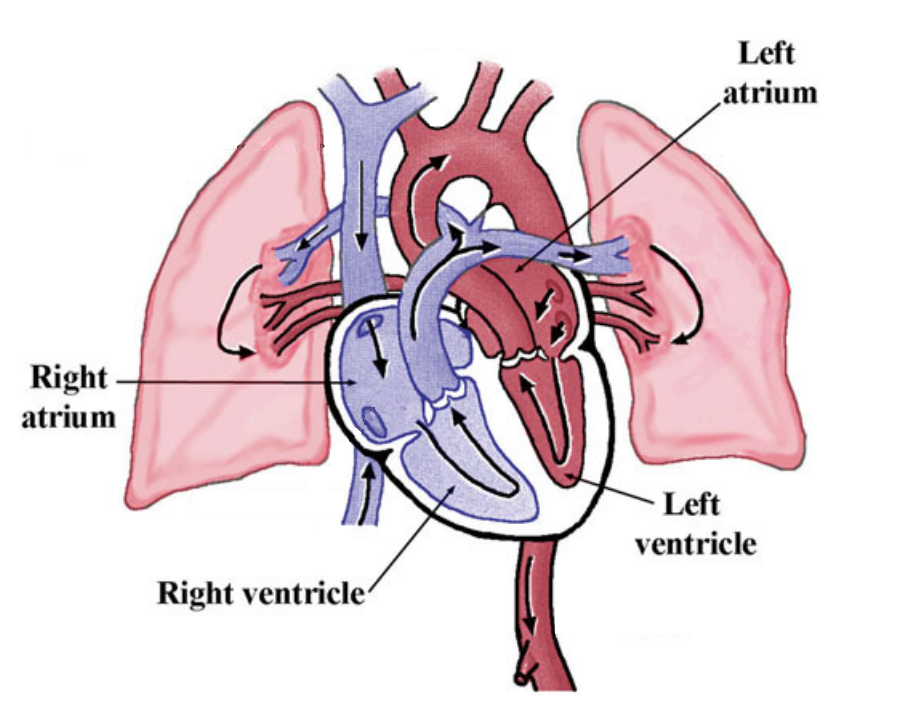
\includegraphics[width=0.5\textwidth]{images/BasicAnatomy.png}
    \caption{The anterior view of a simplified blood flow schematic of the heart and lungs. \citep{BasicAnatomy}}
        \label{fig2.1}
\end{SCfigure}
\begin{SCfigure}[0.5][h!]
    \centering
    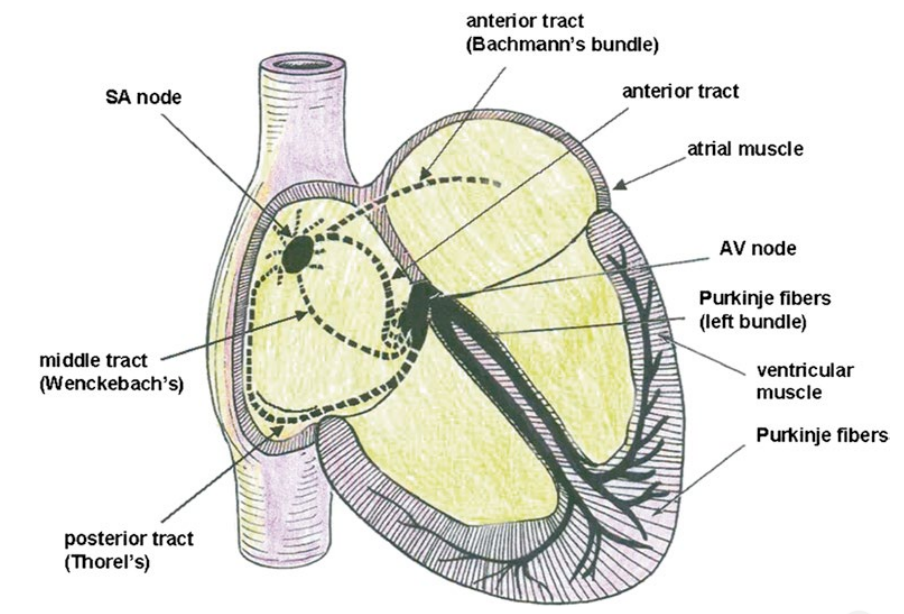
\includegraphics[width=0.7\textwidth]{images/ConductionSystem}
    \caption{Conduction System of the heart. The key areas of interest are the SA (sinoatrial) node and the AV (atrioventricular) node. Signals originate in the SA node and terminate in the muscular tissue via the Purkinje fibres. \citep{ConductionSystem}}
        \label{fig2.2}
\end{SCfigure}
The contracting phase of the cardiac cycle is known as systole, the relaxation phase where the ventricles refill is the diastole. The coordination of the millions of myocardial cells is required for effective pumping. This coordination is governed by the conduction system of the heart (see figure \ref{fig2.2}) and is achieved via electrical excitations, known as action potentials, which propagate through the heart's conductive cells thus activating the cardiac myocytes for muscular contractions. The action potentials of one cell conduct to the next via gap junctions (see section \ref{gapjunctions}). Originating from the sinoatrial node (SAN) in the right atrium, the signal propagates to the atrioventricular node (AVN) and then to to the ventricular muscle via the bundle of His and Purkinje fibres. \par

The main area of interest in this paper is the pacemaker function of the heart, this is controlled by the SAN-AVN complex. As such, the focus of the remainder of this section will be on the right atrium and the ventricular response of the heart will be largely ignored.

\subsection{Cardiac Electrophysiology}
The normal functioning of the heart is dependent on the coordinated contractions of the cardiac myocytes, the muscle cells within the heart. They function due to the charge difference across the membrane of the cell. This creates an electric potential known as the membrane potential. The contraction of the cells is stimulated by an action potential, a depolarizing transitory membrane potential, this interaction is explained in more depth in sections \ref{cellelectro} \& \ref{gapjunctions}. This stimulation originates from the SAN which acts as the pacemaker of the heart. \par

This extracellular potential can be measured using an electrocardiogram (ECG) which comprises of multiple electrodes placed at standardised positions on the body. A basic ECG can be acquired with three electrodes, known as the Einthoven leads, which are placed on the left arm $\Phi_L$, right arm $\Phi_R$, and the left foot $\Phi_F$. The potentials between these electrodes are known as Einthoven standard limb leads and are defined as
\begin{equation}
    \begin{split}
        & V_I = \Phi_L - \Phi_R \\
        & V_{II} = \Phi_F - \Phi_R \\
        & V_{III} = \Phi_F - \Phi_L
    \end{split}
    \label{Eq2.1}
\end{equation}
The Einthoven method assumes the heart is located at the centre of a homogeneous spherical conductor as shown in figure \ref{fig2.3}. Additional leads can be used to obtain more complete ECGs. These additional leads are known as augmented leads ($aV_R, aV_L, aV_F$), which bisect the Einthoven leads, and precordial leads ($V_1, ..., V_6$), which are placed at locations on the chest. The ECG that is typically seen is the voltage over time measured by lead I and is shown in figure \ref{fig2.3}.
\begin{figure}[H]
    \centering
    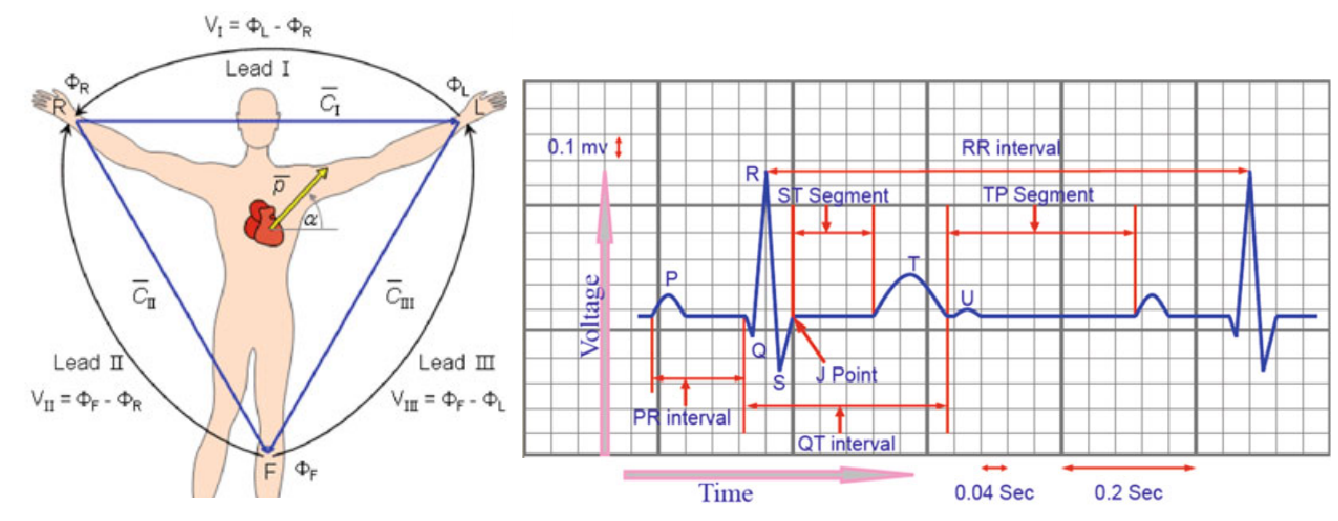
\includegraphics[width=1\textwidth]{images/ECGbasics.png}
    \caption{A Schematic view of Einthoven standard limb leads (left) and a schematic view of a normal lead I ECG (right). \citep{ecg}}
    \label{fig2.3}
\end{figure}
As can be seen in the lead I ECG, the voltage changes as the heart goes through a cardiac cycle. Each deflection from the resting potential corresponds to a different phase of the cycle. The P wave is associated with atrial depolarisation and is the main area of interest of this paper, the atrial repolarisation is obscured by the much larger QRS complex. The QRS complex corresponds to the ventricular contraction. The T wave is the result of the ventricular repolarisation. The relation of each deflection on an ECG with the cardiac cycle can be seen on a Wiggers diagram (figure \ref{fig2.4}).\par
\begin{figure}[H]
    \centering
    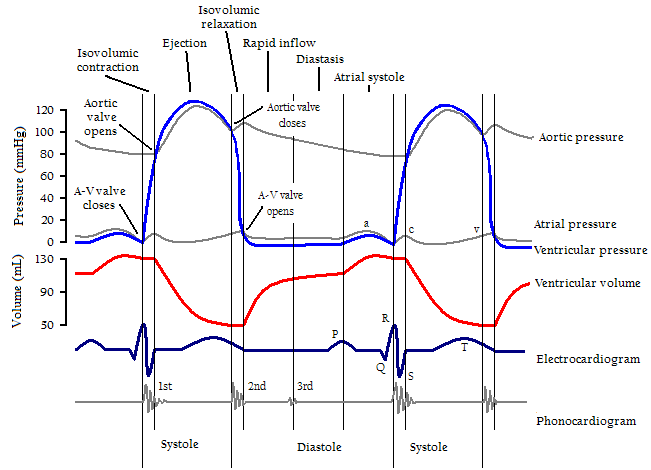
\includegraphics[width=0.95\textwidth]{images/Wiggers_Diagram.png}
    \caption{Wiggers diagram of a cardiac cycle. \citep{wiggers}}
    \label{fig2.4}
\end{figure}
The P wave is of particular interest in this paper as it can be thought of as the average action potential across the atria. The action potentials of the cells at various locations within the heart are different based on their function. For the P wave the cells of interest are nodal cells and the atrial conduction cells.

\subsection{Single Cardiac Cell Electrophysiology} \label{cellelectro}
Ventricular and atrial action potentials are controlled by voltage gated ion channels and can be described as a five phase process as shown in figure \ref{fig2.5}. \par
\begin{SCfigure}[0.5][h!]
    \centering
    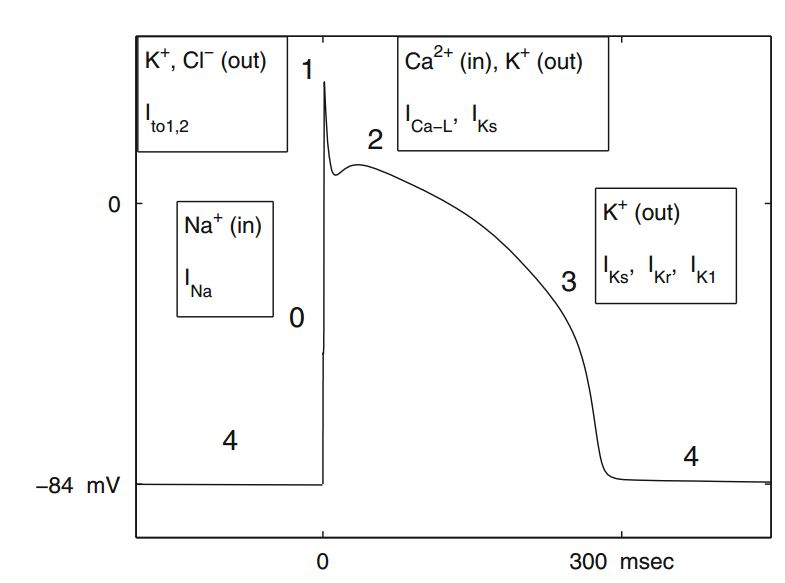
\includegraphics[width=0.7\textwidth]{images/actionpotential.png}
    \caption{Schematic plot of an atrial conduction cell action potential with phases 0 through 4. The ions associated with each phase are shown. \citep{ecg}}
    \label{fig2.5}
\end{SCfigure}
\textbf{Phase 0: Depolarisation.} Rapid depolarisation due to the opening of $Na^+$ channels and the rapid uptake of $Na^+$ by the cell. \par
\textbf{Phase 1: Peak.} The deactivation of the $Na^+$ channels and the release of $K^+$ \& $Cl^-$. \par
\textbf{Phase 2: Plateau.} A balanced flow of inward $Ca^{2+}$ and outward $K^+$. It is these calcium ion currents that cause the cardiac action potentials to have longer duration than neuronal action potentials. \par
\textbf{Phase 3: Repolarisation.} $Ca^{2+}$ channels close and more $K^+$ channels open. \par
\textbf{Phase 4: Resting.} The cell is restored to its resting potential until stimulated by an external source. \par
Nodal cells function slightly differently, these cells spontaneously rise to the threshold voltage of the $Ca^{2+}$ channels allowing them to autonomously activate. There is no phases 1 or 2 in nodal cells as the depolarisation is caused by comparatively slow $Ca^{2+}$ channels due to the lack of fast $Na^+$ channels in SAN cells. The opening of the voltage-gated $K^+$ channels cause the repolarisation phase 3. This reaches a minimum potential whereby the channels close and the cell slowly repolarises due to what are described as leaky $Na^+$ channels \citep{ConductionSystem}. Due to this spontaneous excitation, the SAN has the most rapid and regular excitation causing it to govern the heart rate via a principle known as overdrive suppression. In a normal healthy heart this excitation rate is between 60-100 beats/min. The conduction cells between the SA and AV node cells also have a degree of spontaneous excitation but at a slower rate than the nodal cells, meaning the nodes control excitation rate. A schematic of a nodal action potential can be seen in figure \ref{fig2.6}. \par
\begin{SCfigure}[0.95][h!]
    \centering
    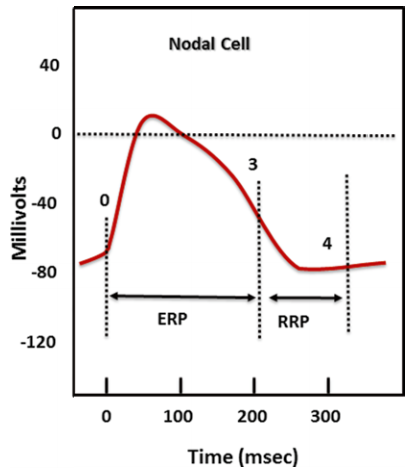
\includegraphics[width=0.4\textwidth]{images/nodalpotential.png}
    \caption{A schematic of the action potential of a nodal cell. Phases 1 and 2 are not observed. There is no stable resting potential. The refractory period for nodal cells is limited by the potential for opening $Ca^{2+}$ channels. \citep{ConductionSystem}}
    \label{fig2.6}
\end{SCfigure}
%push onto next page
\newpage
A typical cardiac conduction cell has a resting membrane potential ($V_m$) between -80 and -90 mV. This is found using the Goldman-Hodgkin-Katz (GHK) equation;
\begin{equation}
    V_m = (2.3R*T/F)*log_{10}\frac{P_K[K]_o + P_{Na}[Na]_o + P_{Cl}[Cl]_i + P_{Ca}[Ca]_i}{P_K[K]_i + P_{Na}[Na]_i + P_{Cl}[Cl]_o + P_{Ca}[Ca]_o}
    \label{eq2.2}
\end{equation}
where $P$ is the permeability, $[X]_x$ is the intracellular and extracellular concentrations of ion X, $T$ is the temperature, $R$ is the ideal gas constant and $F$ is Faraday's constant. The term for calcium, however, is regularly ignored due to the comparatively low concentrations of the ion, as shown in table \ref{table2.1}. When calculated with the GHK equation, typical values found for the resting potential lie around -84 mV. \par
\begin{table}[h!]
\centering
 \begin{tabular}{||c c c||} 
 \hline
 Ion & Intracellular Concentration (mM) & Extracellular Concentration (mM) \\ [0.5ex] 
 \hline\hline
 Na & 5-34 & 140 \\ 
 \hline
 K & 104-180 & 5.4 \\
 \hline
 Cl & 4.2 & 117 \\
 \hline
 Ca & - & 3 \\
 \hline
\end{tabular}
\caption{Typical resting ion concentrations for a typical cardiac cell. \citep{ionconc}}
\label{table2.1}
\end{table}
Individual cell types have slightly different observed properties which govern how the signal propagates through the heart. Table \ref{table2.2} and figure \ref{fig2.7} detail the action potentials of the cells of interest in this paper.
\begin{table}[h!]
\centering
 \begin{tabular}{||c c c c c c||} 
 \hline
 Cell & DP (mV) & Upstroke (mV/ms) & Peak (mV) & APD (ms) & PV (mm/ms) \\ [0.5ex] 
 \hline\hline
 SAN & -50,-60 & 1-10 & 30 & 100-200 & 0.03-0.05 \\ 
 \hline
 Atria & -80 & 100-200 & 30 & 100-200 & 0.3-0.7 \\
 \hline
 AVN & -60,-70 & 5-15 & 20 & 100-300 & 0.1 \\
 \hline
\end{tabular}
\caption{Average values of diastolic potential (DP), upstroke velocity (Upstroke), peak potential (Peak), action potential duration (APD) and propagation velocity (PV) for the cells of interest \citep{ecg}.}
\label{table2.2}
\end{table}
\begin{SCfigure}[0.9][h!]
    \centering
    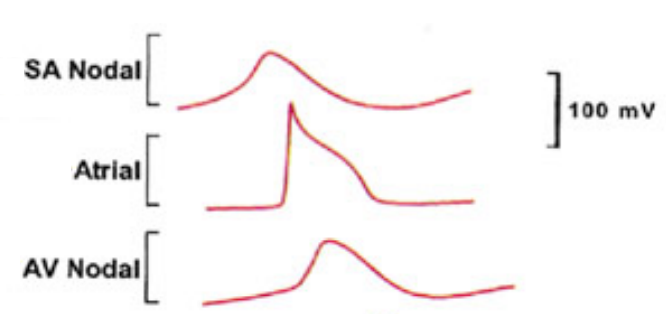
\includegraphics[width=0.4\textwidth]{images/cardiacactionpotentialregions.png}
    \caption{Schematic diagram of typical action potentials observed for the cells of interest. The duration of the potential is approximately 0.3 seconds. \citep{ecg}}
    \label{fig2.7}
\end{SCfigure}

\subsection{Gap Junctions \& Multiple Cells} \label{gapjunctions}
Cells are connected end to end by intercalated disks holding the cells together. Adjacent to these disks are gap junctions. Gap junctions allow action potentials to spread from one cell to the next via low-resistance pathways formed by protein connections on the disks \citep{gapjunctions}. It takes approximately 30 ms for excitation to spread between the SAN and AVN and activation occurs over 70-90 ms. Gap junctions are key factors in heart disease; issues with gap junctions have been linked to arrhythmia, ischemia and heart failure.\par

Gap junctions are more abundant in the connections between the ends of the cells than the sides allowing for faster propagation along a fibre than perpendicular to it, however, fibres in the atria are very irregular. Due to this anisotropy it is impractical to model gap junctions explicitly. Instead a continuum approach is usually used in mathematical models and the propagation between cells is described by diffusion of ions through a uniform space. More sophisticated models have described this propagation using 3 dimensional tensor mathematics \citep{unansweredquestions}. \par

One key observation to be made when considering activation propagation across multiple cells is that the action potential duration is much longer than the time taken to propagate across the atrium \citep{ecg}. The action potential lasts approximately 0.3 seconds but only 0.03 seconds for the excitation to spread between the SAN and AVN. This means that the whole medium is excited at the same time suggesting that it is the trailing edge of the wave front which causes re-entry in the presence of blockers.

\subsection{Refractory Periods \& Re-entry}
\label{section2.4}
An important property of individual cells is that they have a refractory period after excitation in which the cell recovers. One effect of this is to prevent rapid stimulation; if rapid stimulation occurred continuously the contraction ability of cells would be inhibited reducing cardiac output. This property prevents rapid stimulation propagating through the tissue, this has important effects on re-entry. \par

Re-entry is where a propagating wave is self-sustained in the tissue. This may occur as a spiral wave propagating around a blocker (see figure \ref{fig2.8}). The refractory period of cells helps prevent re-entry by not allowing cells to re-excite for a period of time, however, in the case of a uni-directional current block the wave can propagate around the block and then re-enter through the opposing side allowing enough time for cell recovery. Re-entry is a primary cause of many arrhythmias and has been linked to many cardiac diseases, understanding its effects are key to developing treatments. \par
\begin{figure}[h]
    \centering
    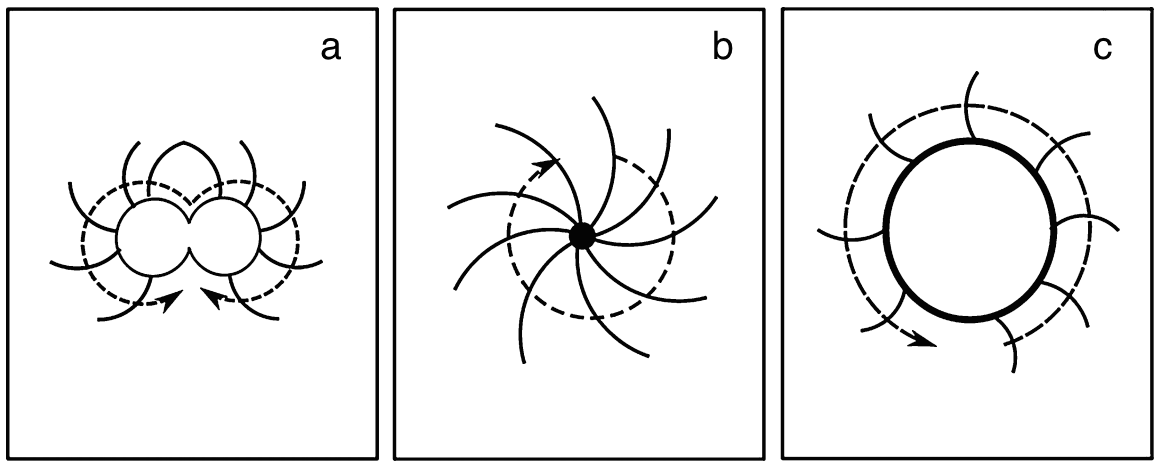
\includegraphics[width=0.9\textwidth]{images/reentry.png}
    \caption{Re-entry schematic. Dotted arrow shows wave propagation direction. (a) Shows two waves rotating in opposite directions around a blocker, if uni-directional the wave can back-propagate through the block. (b) Shows a spiral wave around a central node. (c) Shows a wave propagating around a large structural obstacle. \citep{phdpaper}}
    \label{fig2.8}
\end{figure}

\subsection{Cardiac Arrhythmias and Diseases}
Arrhythmias refer to either the lack of rhythm or irregular rhythm of the heart beat. Irregular contraction can lead to restricted output or even death. The majority of cardiac conditions are the result of, or lead to, arrhythmias. Bellow are some of the common arrhythmia related diseases.
\subsubsection{Tachycardia}
Tachycardia is the fast reactivation of the heart, resulting in a faster than normal resting heart rate. Commonly the result of re-entrant waves due to the presence of uni-directional blockers in the conductive tissue. Associated with reduced cardiac output and have a chance to develop into fibrillation.
\subsubsection{Bradycardia}
Bradycardia refers to the slow reactivation of the heart. Associated with atrioventricular nodal blocks and underlying problems with the heart rate regulatory system. Bradycardia results in reduced cardiac output significantly reducing nutrient and oxygen supply to organs.
\subsubsection{Ischemia}
Ischemia is the result of a portion of cell death within the heart tissue, an antisymmetric omni-directional block. These regions do not contract or pass conduction signals, resulting in reduced cardiac output. If of significant size this can block wave propagation resulting in re-entry potentially causing tachycardia and fibrillation.
\subsubsection{Fibrillation}
The fast and irregular activation of the heart is known as fibrillation. Associated with the re-entry of spiral waves, fibrillation has a serious effect on cardiac output and coordination. Atrial fibrillation can predispose ventricular fibrillation, commonly known as a heart attack, and death.

%---------------------------------------------------------------------------%
\newpage
\section{Models}
    \label{section2.2}
Transmembrane potentials are due to ion flux accross the membrane. These ion fluxes can be described by the Nernst-Plank equation
\begin{equation}
    J_{total} = J_{diff}+J_{elec} = -D\bigg(\nabla c + \frac{zF}{RT}c\nabla u\bigg)
    \label{nerstplankeq}
\end{equation}
where $J_{total}$ is the total ion flux, $J_{diff}$ is the diffusion flux, $J_{elec}$ is the electric flux, $D$ is the diffusion coefficient and $c$ is the concentration of the ion, $R$ is the ideal gas constant, $T$ is temperature, $F$ is Faraday's constant and $u$ is the electric potential. The Nernst-Plank equation is derived from Fick's law and the Einstein relation, a full derivation can be found in appendix \ref{appendixNPE}. \par
The Nernst-Plank equation can be applied to cellular geometries and used to form the Goldman-Hodgkin-Katz (GHK) current-voltage relation (equation \ref{GHKcvr}) which is used to calculate the ion concentrations and currents discussed in section \ref{cellelectro}
\begin{equation}
    I=P\frac{z^2F^2}{RT}v\frac{c^i-c^eexp\big(\frac{-zvF}{RT}\big)}{1-exp\big(\frac{-zvF}{RT}\big)}
    \label{GHKcvr}
\end{equation}
where $I$ is the electric current density, $P$ is the permeability of the membrane to the ion, $z$ is the valence of the ion and $v = u(0)-u(L) = u_i-u_e$ where $L$ is the membrane length. $c$ is the ion concentration and the $i$ and $e$ notation is used to indicate intra and extracellular values. A full derivation of the GHK current-voltage relation can be found in appendix \ref{appendixGHK}.\par
These equations fundamentally describe the transmembrane potential actions of interest and most models are based of the fundamental relations described by these equations.

\subsection{Equivalent Circuit Model}
An alternative approach to describing the transmembrane potential is by considering electrical circuits. Cells can be described simply as an insulating lipid bilayer membrane with voltage controlled pores known as ion channels. The insulating membrane separates intra and extracellular ion concentration acting as a basic capacitor. The ion channels themselves can be most simply described as resistors (see figure \ref{fig3.1}). If the membrane capacitance ($C_m$) is constant, the current across the membrane ($I_{cap}$) can be described as
\begin{equation}
    I_{cap} = \frac{dQ}{dt} = C_m\frac{dv}{dt}
\end{equation}
were $Q$ is the charge and $v$ is the potential across the membrane. By Kirchhoff's law the total current applied to the membrane, $I_{app}$ is the sum of the membrane capacitance current $I_{cap}$ and the current through the ion channels $I_{ion}$.
\begin{equation}
    I_{app}=C_m\frac{dv}{dt}+I_{ion}
\end{equation}
The structure of the total $I_{ion}$ current is dependent on the specific model employed.

\subsection{Ion Channel Gating}
The current through an ion channel, in general, can be modelled as a product of a function of the number of open channels, $g(v,t)$, and a function of the channels current-voltage relation, $\phi(v)$. $\phi(v)$ can be modelled by various equations as discussed in section \ref{ccmm} on membrane models. The functions $g(v,t)$ can be found experimentally via voltage clamp methods where an external current is applied to a cell to balance the membrane current in a way that keeps the membrane potential $v$ fixed.\par

It is found that the function $g(v,t)$ is related to the number of subunits that make up the ion channel and the kinetics of those subunits. Subunits are the individual complex proteins that make up the channels and pumps. The Hodgkin-Huxley model takes this concept and couples the equivalent circuit model with these gating functions.

\subsection{Hodgkin-Huxley Model}
One of the most celebrated action potential models, the Hodgkin-Huxley (HH) model, combines the equivalent circuit model with gating functions of the form
\begin{equation}
    \frac{dw}{dt} = \frac{w_\infty - w}{\tau_w}
\end{equation}
where $w$ is the gating variable, $w_\infty$ is the equilibrium state and $\tau_w$ is the time constant. \par

The HH model simulates nerve action potentials by using 3 gating variables $m$, $h$ and $n$ to describe the system of the sodium, potassium and leakage currents that make up nerve axon action potentials.
\begin{equation}
    \begin{split}
        & C_m\frac{dv}{dt} + I_{ion}(v,m,h,n) = I_{app} \\
        & \frac{dm}{dt}=\frac{m_\infty(v) - m}{\tau_m(v)} \\
        & \frac{dh}{dt}=\frac{h_\infty(v) - h}{\tau_h(v)} \\
        & \frac{dn}{dt}=\frac{n_\infty(v) - n}{\tau_n(v)} \\
    \end{split}
\end{equation}
and the $I_{ion}$ current is the sum of the individual ion currents and leakage current $I_L$.
\begin{equation}
    I_{ion}=I_{Na}+I_{K}+I_{L}
\end{equation}
It is found that the gating variables are dependent on the number of subunits involved in each channel and their kinetics. The HH approach can be expanded to take into account the larger ionic system involved with cardiac action potentials, leading to a large variety of models for each of the unique cell types of the heart.

\subsection{Cardiac Cellular Membrane Models}
\label{ccmm}

Sophisticated models of individual cell types with a focus on the ionic currents involved have been developed. One of the vital areas of the heart is the sinoatrial node, SAN, which acts as the natural pacemaker. Detailed membrane models have been produced for various animals with noticeable examples being Zhang et al. model of rabbit SAN cells \citep{zhangsan} and Severi et al. model which focuses on calcium ion handling and inhibition which is crucial to the unique plateau in phase 2 of the cardiac cell action potential \citep{severisan}. \par

Atrial tissue models have also been developed such as Nygren et al. human right atrial model which is based on voltage clamp data of isolated cells \citep{nygrenatrial}. Combining HH type equations with a fluid model for intracellular ion movement within the cytoplasm means this model is a very accurate single cell action potential model. The Nygren model and other similar models are embellishments of DiFrancesco and Noble's models of cardiac electrical activity \citep{DiFrancescoNoble}. These models are accurate representations of single cell systems and ion behaviour. \par

The first ventricular model was developed by Beeler and Reuter \citep{beelerreuter}. It was based on the HH model but introduced dynamics necessary to model the effects of calcium ions which are crucial to cardiac action potentials. Many other ventricular models have been developed of varying complexity, a collection of these are shown in table \ref{ventmodletable}. \par

The Beeler and Reuter model along with the Luo and Rudy model were the early attempts to consider calcium ion dynamics. Later models such as Puglisi's model and Shannon's model included more detailed descriptions of the calcium dynamics. Further complexity has been included in more recent models for sodium and potassium ion dynamics and O'Hara and Rudy's model of human ventricular myocytes is particularly detailed.

\begin{table}[h!]
\centering
    \begin{tabular}{||c c c||} 
        \hline
        Model & Species & Equations \\ [0.5ex] 
        \hline\hline
        Beeler \& Reuter \citep{beelerreuter} & Mammalian & 8 \\
        \hline
        Luo \& Rudy \citep{luorudy} & Guinea Pig & 8 \\
        \hline
        Priebe \& Beuckelmann \citep{priebe} & Human & 22 \\
        \hline
        Pandit et al. \citep{pandit} & Rat & 26 \\
        \hline
        Jafri, Rice \& Winslow \citep{JRW} & Guinea Pig & 31 \\
        \hline
        O'Hara \& Rudy \citep{ohararudy} & Human & 41 \\
        \hline
        Shannon et al. \citep{shannon} & Rabbit & 46 \\
        \hline
        Cortassa et al. \citep{cortassa} & Mammalian & 50 \\
        \hline
    \end{tabular}
\caption{A table of some of the most popular ventricular myocyte models. The models are of varying complexity and for different species' dynamic systems.}
\label{ventmodletable}
\end{table}

\subsection{Lightweight Ionic models}
Many of the individual cellular models already mentioned are highly sophisticated and complex. They describe individual cell ion dynamics very well, however, the models themselves are large and mathematically cumbersome, made up of many coupled equations. In order to investigate large multicellular geometries over long temporal scales a reduced model is necessary. These reduced models accurately provide an action potential but without the complex sub-cellular dynamics. This allows for accurate action potential simulation without the computational cost associated with complex models.
\subsubsection{Fitzhugh-Nagumo and Cubic-Like Models}
The Fitzhugh-Nagumo (FN) model is one such example of a lightweight ionic model and is based on a pair of ODEs of the normalised variables $u$, the transmembrane potential, and $v$, the gating variable \citep{fitzhugh}. The equations are based around the form
\begin{equation}
    \begin{split}
        & \frac{du}{dt} = f(u,v) \\
        & \frac{dv}{dt} = g(u,v)
    \end{split}
    \label{FNeq}
\end{equation}
The FN model is one example of cubic-like reduced ionic models and is of the general form 
\begin{equation}
    \begin{split}
        & f(u,v) = -ku(u-a)(u-1)-v \\
        & g(u,v) = \epsilon(u-bv) \\
    \end{split}
\end{equation}
Other cubic-like models have been developed such as the Aliev-Panfilov model \citep{alievpanfilov} and the Mitchell-Schaeffer model \citep{mitchellSchaeffer}. \par

An alternative approach to reduced models is shown in the Fenton-Karma model \citep{fentonkarma}. This consists of three ODEs making up the transmembrane potential, $u$, with two gating variable, $v$ and $w$, as shown in equation \ref{eqFK}.
\begin{equation}
    \begin{split}
        & \frac{du}{dt} = f(u,v,w) \\
        & \frac{dv}{dt} = H(u-u_c)(1-v)/\tau^{-}_{v(u)} - H(u-u_c)v/\tau^{+}{v} \\
        & \frac{dw}{dt} = H(u-u_c)(1-w)/\tau^{-}_{w(u)} - H(u-u_c)w/\tau^{+}{w} \\
    \end{split}
    \label{eqFK}
\end{equation}
where $H$ is the Heaviside function and $f(u,v,w)$ is the sum of the individual membrane ionic currents which can be found experimentally via voltage clamp methods or modelled. \par

Looking at the FN model in more detail, it can be derived from a simple circuit model of a cell membrane. The circuit is made up of a capacitor (current $I_{cap}$) in parallel with a nonlinear current voltage device (current $I_{ion} = F(u)$) and a serial system of a resistor, an inductance, and a voltage source (current $I_0$). Let $u$ equal the transmembrane potential (the difference between the intra, $u_i$, and extra, $u_e$, cellular potentials). Also let $v_R$, $v_L$, and $v_0$ be the resistor, inductor and voltage source potentials. By using Kirchhoff's laws:
\begin{equation}
    \begin{split}
        & I_a = I_{cap} + I_{ion} + I_0 \\
        & u = v_0 + v_L + v_R \\
    \end{split}
\end{equation}
Then by using Ohm's law ($v_R=RI_{ion}$), Faraday's law ($v_L=L\frac{dI_{ion}}{dt}$) and the equation for capacitance ($I_{cap}=C\frac{du}{dt}$) we form
\begin{equation}
    \begin{split}
        & C\frac{du}{dt} = -I_{ion} -F(u) +I_a \\
        & L\frac{I_{ion}}{dt} = u - RI_{ion} - v_0 \\
    \end{split}
\end{equation}
The equation can be made dimensionless by scaling time as $\tau=R_mt/L$, where $R_m=1/F'(0)$. By defining the dimensionless variables as
\begin{equation}
    \begin{split}
        & v(\tau)=u(L\tau/R_m)/u_m \\
        & w(\tau)=R_mI_{ion}(L\tau/R_m)/u_m \\
    \end{split}
\end{equation}
where $u_m$ is the maximum value of $u$. By applying these variables and then defining $\hat v_0=v_0/u_m$, $\hat F(u)=\frac{R_m}{u_m}F(u_mu)$, $\hat I_a=\frac{R_m}{u_m}I_a$, $\gamma = R/R_m$, and $\epsilon = CR^{2}_{m}/L$ gives
\begin{equation}
    \begin{split}
        & \epsilon\frac{du}{d\tau} = -w - \hat F(u) + \hat I_a \\
        & \frac{dw}{d\tau} = u - \gamma w - \hat v_0 \\
    \end{split}
\end{equation}
This is a particular instance of a generalised FN dynamic system
\begin{equation}
    \begin{split}
        & \epsilon\frac{du}{d\tau}=f(u,w) + \hat I_a \\
        & \frac{dw}{d\tau} = g(u,w) \\
    \end{split}
    \label{eqGFN}
\end{equation}

\subsection{Phase Analysis of Fitzhugh-Nagumo Equations}
\begin{figure}[H]
    \centering
    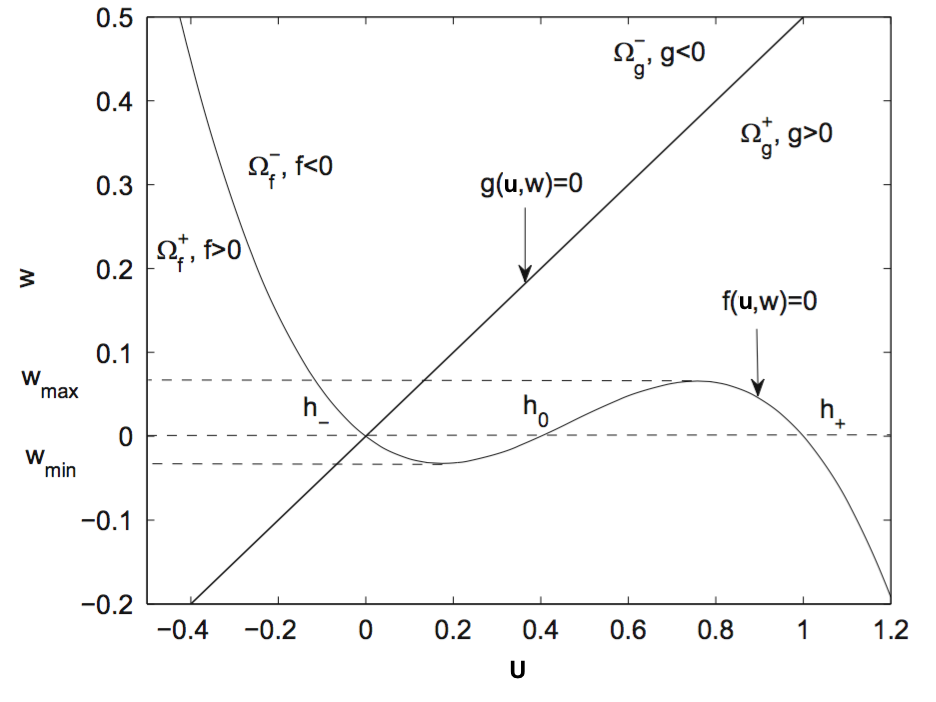
\includegraphics[width=0.8\textwidth]{images/PhasediagramFN.png}
    \caption{$u$ and $w$-phase plane diagram for the FN model. Nullcline intersection points are indicated as $h_-$, $h_0$ and $h_+$. \citep{ecg}}
    \label{fig2b.1}
\end{figure}
To fully understand the behaviour of equation \ref{eqGFN} a phase analysis is necessary. As shown in figure \ref{fig2b.1}, the nullcline $f(u,w)=0$ is a cubic like function with 3 distinct zeros: $h_-$, $h_0$ and $h_+$. The nullcline $g(u,w)=0$ has only one intersection point which is an equilibrium point of the system. As the phase plane trajectory passes across the nullclines it will attempt to move towards this equilibrium point. By choosing various initial conditions, equation parameters and applied current ($\hat I_a$), the generalised FN equation (equation \ref{eqGFN}) shows greatly varying dynamics. \par
For the generalised FN system, stability exists when the phase plane trajectory lies on the upper ($h_+$) or lower ($h_-$) branch of the $f=0$ nullcine while there is instability when the trajectory lies on the middle ($h_0$) branch. There are 3 main situations when manipulating the applied current; when $\hat I_a = 0$, $\hat I_a > 0$, and when $\hat I_a$ is pulsed.

    \subsubsection{Generalised FN with Zero Applied Current}
    With zero applied current the parameters of the equation have a major impact in the phase plane trajectory (figure \ref{fig2b.2}).\par
    If the initial condition $u_0 < h_0$ holds then a sub-threshold response is witnessed as $v$ returns directly to the equilibrium point via the lower branch. This is because within the region $\Omega _{f}^{-} \Omega _{g}^{-}$ the trajectory is above the nullcline $g=0$ which forces the return down $h_-$ to the equilibrium point. Similarly if the parameters start in the $\Omega _{f}^{-} \Omega _{g}^{+}$ region then $g>0$ so initially increases the trajectory across $g=0$ back into the $\Omega _{f}^{-} \Omega _{g}^{-}$ region. \par
    If, however, the initial condition $u_0>h_0$ is chosen then a single action potential can be observed. A clear excitation phase is seen when the trajectory tends to the upper branch. This is followed by a very brief plateau as the trajectory lingers on the upper branch. The gating variable $w$ evolves into an approximate constant, driving the trajectory across the $g=0$ nullcline towards the lower branch, this mimics the recovery phase. The trajectory then relaxes down the lower branch to the equilibrium point. \par
    Alternative to these stable equilibrium situations an unstable equilibrium can be formed. This forms a limit cycle due to periodic solutions. This occurs when the equilibrium point lies on the middle branch as the trajectory of initial excitation starts a second excitation phase generating periodic action potentials. This scenario could potentially be of use in simulating the limited periodic cycles observed on SAN cells.
    \begin{SCfigure}[0.7][h!]
        \centering
        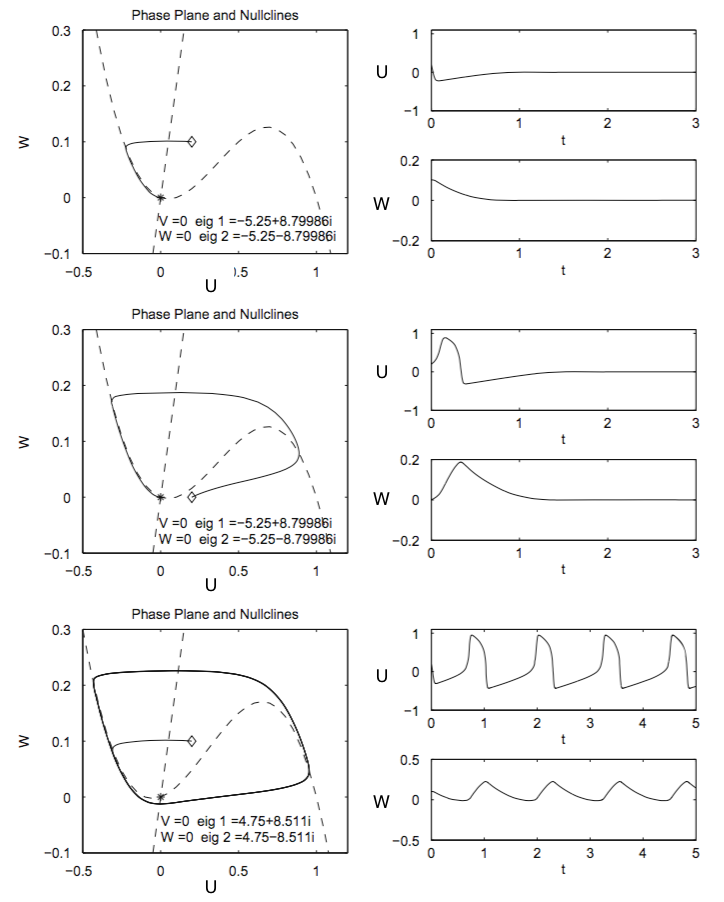
\includegraphics[width=0.65\textwidth]{images/I0cycles.png}
        \caption{Generalised FN model with $\hat I_a = 0, \epsilon=0.01$. For top and middle $f(u,w) = u(u-0.1)(1-u)-w, g(u,w)=u-w/2$. For bottom $f(u,w) = u(u+0.1)(1-u)-w, g(u,w)=u-w/2$. Equilibrium point is marked with a black star, start position is marked with a white diamond. The associated solutions are to the right of the phase diagrams. \citep{ecg}}
        \label{fig2b.2}
    \end{SCfigure}
    \subsubsection{Generalised FN with a Non-zero Applied Current}
    With a small applied constant current an unstable equilibrium can be formed with a periodic limit cycle, similar to the one shown in the bottom panel of figure \ref{fig2b.2}. This is achieved by shifting the $f=0$ nullcline upwards, moving the equilibrium point closer to the upper branch (however still on the middle branch) forcing it to behave as a source point. This yields a periodic action potential where the plateau period can be manipulated by adjusting the equation parameters. \par
    If the applied current is too high the equilibrium point tips over the peak of the $f=0$ nullcline onto the upper branch causing it to behave as a sink point, this attracts the trajectory.
    \begin{SCfigure}[0.7][h!]
        \centering
        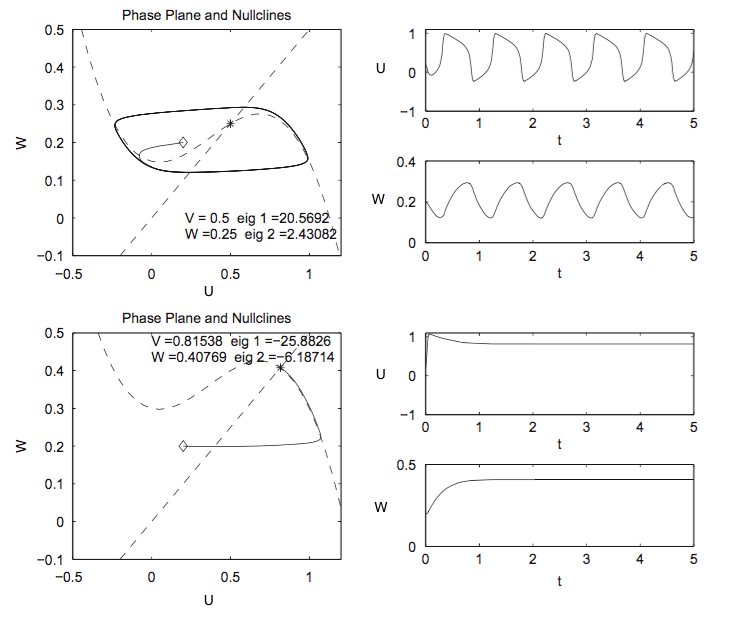
\includegraphics[width=0.63\textwidth]{images/Iposcycles.png}
        \caption{The effects of positive applied potential on the phase plane trajectories of the general FN equation $f(u,w)=u(u-0.1)(1-u)-w, g(u,w)=u-2w$, with $\epsilon=0.01$. Top $\hat I_a = 0.15$, bottom $\hat I_a =0.3$. \citep{ecg}}
        \label{fig2b.3}
    \end{SCfigure}
    \subsubsection{Generalised FN with a Pulsed Non-zero Applied Current}
    In the previous examples a constant applied current has been used. A more physiologically accurate method is to use a pulsed applied current. This simulates the activation of the action potential via a neighbouring cell's pulse or an external stimulus such as a nerve. In this situation the duration that the current pulse is applied for has a significant impact. The applied current pulse temporarily shifts the $f=0$ nullcline upwards (if $\hat I_a >0$) or downwards ($\hat I_a <0$) causing the equilibrium point to shift, this forces the trajectory towards to closest branch. When the pulse is turned off the nullcline returns to the original position. At this time the trajectory is at a point (if correct times and parameters are chosen) which belongs to the excitable region causing an action potential. \par 
    For the generalised FN equation, $f(u,w)=u(u-0.1)(1-u)-w,  g(u,w)=u-w/2$, a positive and negative pulse causes a cathode make and anode break mechanism respectively. A 'make' occurs when an applied current is turned on and a 'break' is where an applied current is turned off. Cathode and anode refer to a negative and positive applied current respectively. The anode break is shown in figure \ref{fig2b.3}. Additional mechanism, known as cathode break and anode make, are observed in more complex systems within cardiac domains. 
    \begin{SCfigure}[0.7][h!]
        \centering
        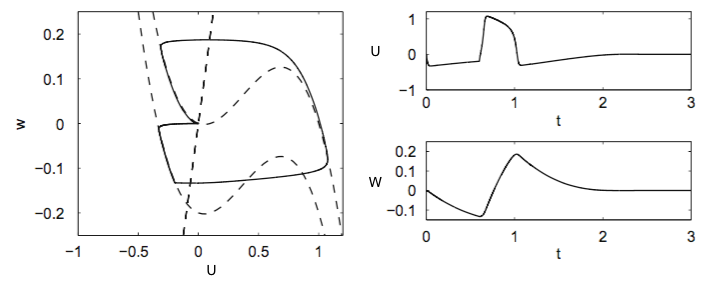
\includegraphics[width=0.65\textwidth]{images/Iperiod.png}
        \caption{A current pulse of $\hat I_a=-0.2$ for 0.6 ms causing an anode break. This action potential is an accurate simulation of an atrial conduction cell. \citep{ecg}}
        \label{fig2b.4}
    \end{SCfigure}
\subsection{Advanced Models}
More advanced models exist that take into account more complex parameters of the system such as rotational anisotropy, conduction fibre structure, cell shape, and the inhomogeneous nature of the intra and extra cellular mediums. \par
The bidomain model is derived from a one dimensional model of an electrical cable. The biodomain model takes the average of all the properties of the cells in the medium rather than modelling each cell individually \citep{bidomain}. The main problem the bidomain model tackles is the anisotropy of electrical conductivity. Within cardiac tissue there is unequal anisotropy ratios for the conductivities parallel and perpendicular to the fibres within the intra and extra cellular mediums. For cardiac tissues the ratio for intracellular space is 10:1, while in extracellular space it is 5:2 \citep{bidomainans}. This anisotropy can effect the action potential in many ways such as the distribution of the transmembrane potential \citep{disttrans}, the magnetic field produced by the propagating wave \citep{magfield}, and the effect of electric shocks on the transmembrane potential \citep{shocks}. \par 
Although detailed, this model is also mathematically cumbersome with the average simulation taking up to 2 days on a 32 processor computer \citep{monodomain}. It is regularly simplified by removing the unequal anisotropy of the intra and extra-cellular domains, this is known as the monodomain model \citep{monodomain}. The monodomain model is more computationally lightweight and does ignore the large difference in anisotropy of the mediums, however, the propagation of activation has been reported to being only 2\% faster for the monodomain model \citep{monodomain}. It has also been reported by the same group that ECGs computed using both models are visually indistinguishable suggesting that this anisotropy can be ignored and effective simulation can still be achieved. The same argument has been used for ignoring the anisotropy in cubic-like models.
\begin{figure}[H]
    \centering
    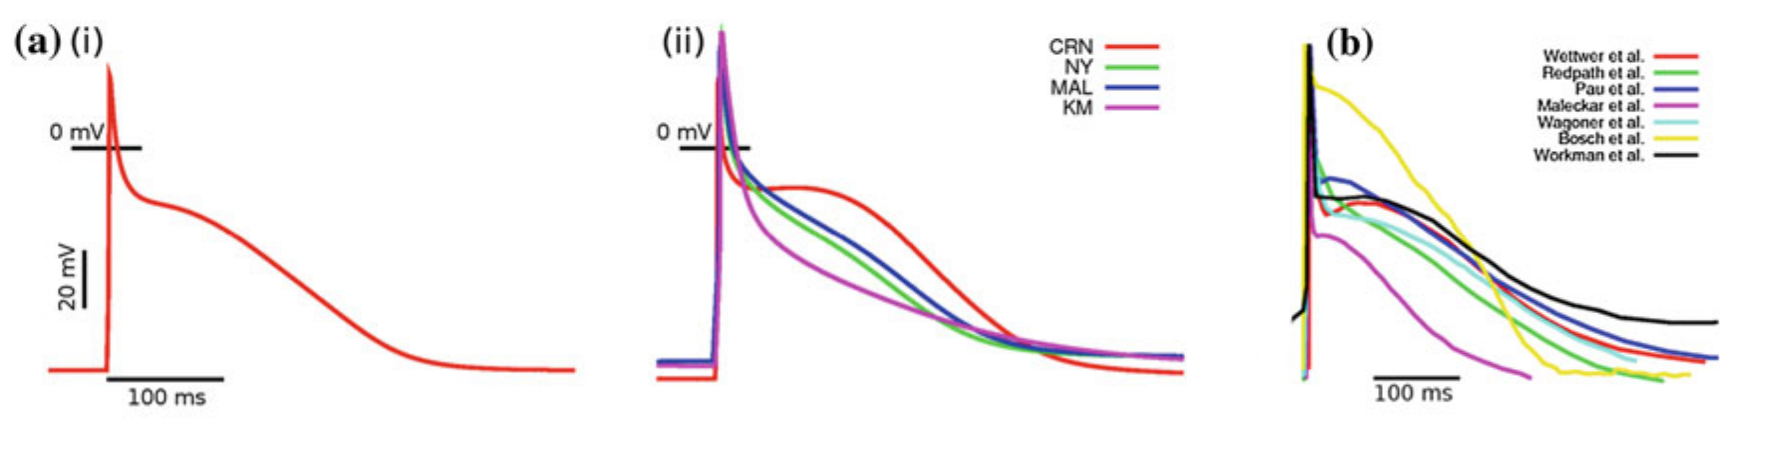
\includegraphics[width=0.9\textwidth]{images/APmodels.png}
    \caption{The (a) panels show a variety of advanced models and the (b) panels show a collection of experimental measurements. (i) shows one of the most detailed models known as the MCZ model by M. Colman \citep{phdpaper}. It is clear that experimental and modelled potentials vary significantly. \citep{phdpaper}}
    \label{fig2b.5}
\end{figure}
%---------------------------------------------------------------------------%
\newpage
\section{Electronic Model}
    \label{section3}
Cells can be simply described as an insulating lipid bilayer with voltage controlled ion channels. As such, they can be described simply via equivalent circuit models, the simplest of such is modelling the membrane as a capacitor and the ion channels as resistors (see figure \ref{fig3.1}). To electronically model action potentials however, a more complex circuit is needed as ion channels do not behave as linear resistors. Instead a channel is modelled as a non-linear current voltage device. \par

The Bonhoeffer-Van der Pol (BVP) electronic model of a single cell action potential is one of the simplest ways to achieve this. In the BVP model the non-linear current voltage device is created by a series voltage source and diode in parallel to an inductor and resistor (see appendix \ref{appendixVDP}). The BVP model was expanded in the original development of the FN model to simulate a nerve axon \citep{fitzhughnagumo}. This was achieved by coupling BVP circuits in a linear fashion as discussed in appendix \ref{appendixVDP}. \par 

A modern simple alternative to the non-linear current voltage devices is to use transistors to control the gating of the simulated ion channels. One circuit that can be accurately described by a FN equation is a three transistor model described by Lancaster and Hellen \citep{3transistor}. This model (shown in figure \ref{fig3.4}) simulates a self exciting cell action potential which has a very similar membrane potential output as predicted by FN equations, where the capacitor voltage represents the membrane potential and the transistor base voltage is the inhibitory variable. \par

\begin{figure}[H]
    \centering
    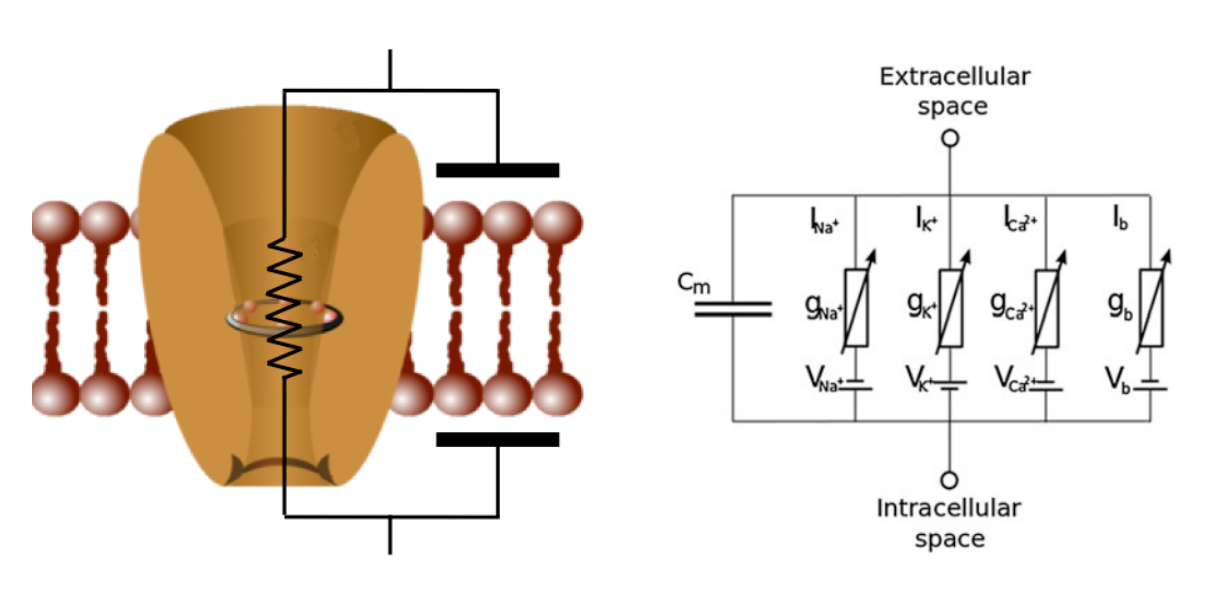
\includegraphics[width=0.8\textwidth]{images/simpleelectronic.png}
    \caption{Left: A simple equivalent circuit model for a cell membrane and ion channel. The system can be represented as a parallel RC circuit \citep{simpleelectronic}. Right: The RC model applied to a cardiac cell where the major ion channels of interest are included. Voltage variable resistors are used to act as the voltage gated ion channels. \citep{phdpaper}}
    \label{fig3.1}
\end{figure}

\begin{SCfigure}[0.9][h!]
    \centering
    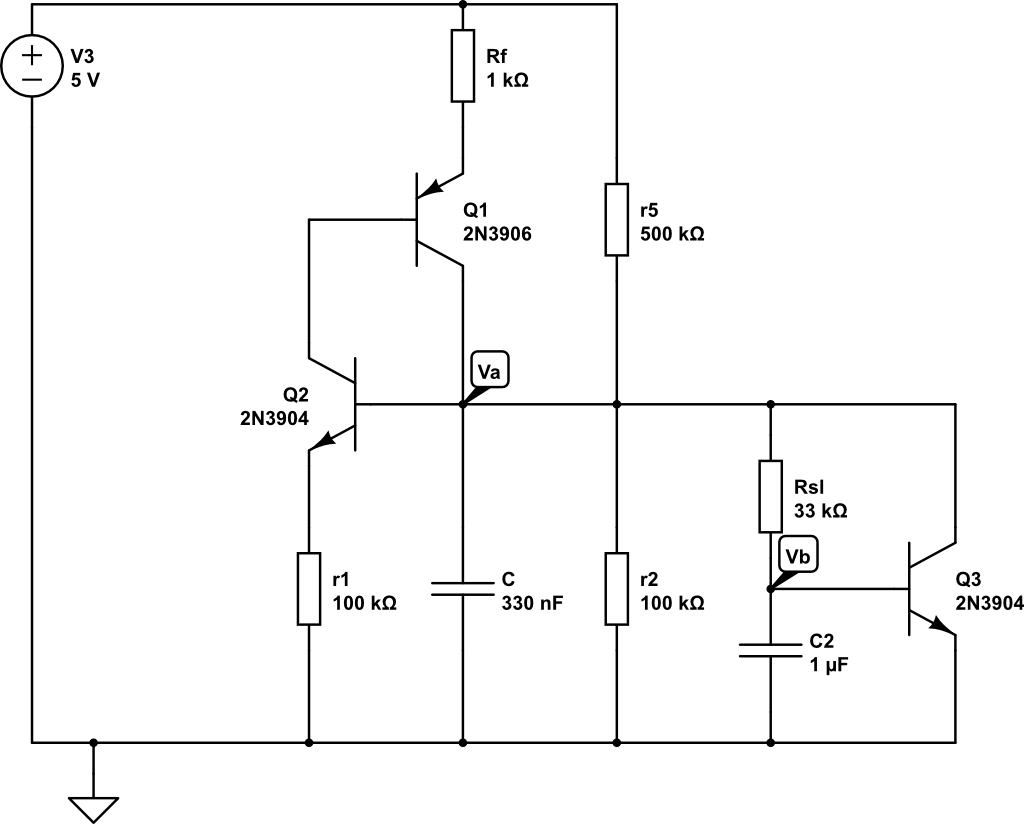
\includegraphics[width=0.5\textwidth]{images/3-transistor-circuit.png}
    \caption{A circuit diagram of the 3 transistor cell model with components identified. $V_a$ is the membrane potential and $V_b$ the inhibitory variable. The two left hand transistors are responsible for the fast-response positive feedback required for the depolarisation phase. The final transistor is responsible for the inhibitory variable.}
    \label{fig3.4}
\end{SCfigure}

\subsection{Electronic Model of an Isolated Cell}
Using the three transistor circuit shown in figure \ref{fig3.4} we computationally simulated the circuits output. The circuit shows a self exciting action potential which can be used to simulate a single excitable cell.
\begin{figure}[H]
    \centering
    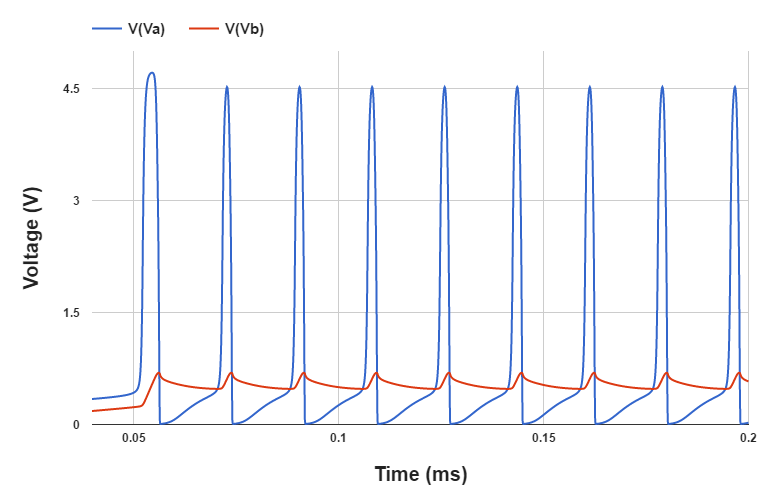
\includegraphics[width=0.7\textwidth]{images/singlecellelec.png}
    \caption{The simulated output of voltmeters placed at positions $V_a$ (the membrane potential) and $V_b$ (the inhibitory variable) shown in figure \ref{fig3.4}.}
    \label{fig3.5}
\end{figure}

\subsection{2D Electronic Model}
By combining these individual 'cells' together in a ring, we can simulate a 2D 'slice' of the atrium. We first simulated this circuit computationally and then created the physical circuit to measure via an oscilloscope, a photo of the full circuit and a full circuit diagram can be seen in appendix \ref{appendixcircuit}. 6 individual cells were used in a ring with the first cell acting as the SAN and each neighbouring cell receiving the output of the previous cell via a resistor (which acts as the extra-cellular diffusion time) as its stimulation current. The final cell receives two inputs simultaneously exciting it. The final cells excitation does not propagate back round as each of its neighbours are in a relaxation state and unable to be excited again, this terminates the current. A regular pulse is observed.
\begin{figure}[H]
    \centering
    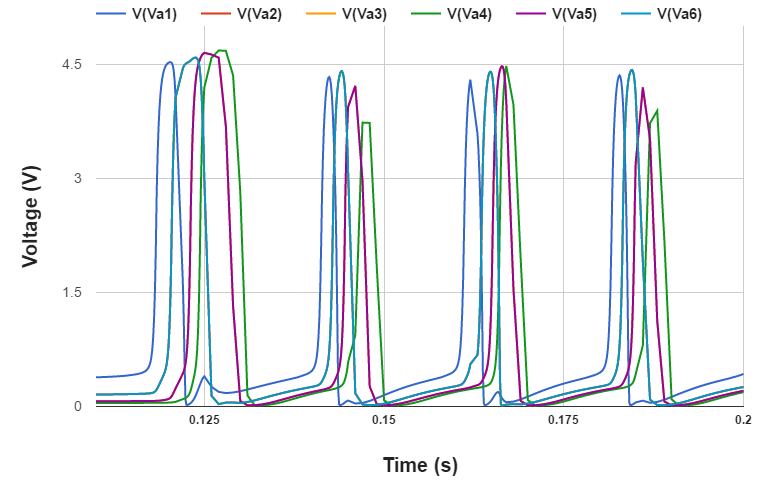
\includegraphics[width=0.7\textwidth]{images/6cellnoblock.png}
    \caption{The simulated output of voltmeters placed at positions $V_a$ (the membrane potential) in figure \ref{fig3.4} for cells 1 though 6 in the ring network shown in appendix \ref{appendixcircuit}.}
    \label{fig3.7}
\end{figure}


\subsection{Simulation of Re-entrant Tachycardia}
As shown in the 2D 6 cell circuit diagram shown in appendix \ref{appendixcircuit}, two switches and a diode can be added between each cell. The switch parallel to the diode can be opened to create a uni-directional blocker and thus simulate tachycardia. The blocker stops current flowing in the forward direction. \par

As an example, opening the switch between cells 6 and 5 (numbering clockwise) means cell 4 does not excite via the forward propagation. Instead, it remains relaxed allowing the AVN cell (cell 3) to excite it. In turn cell 5 has relaxed by this point allowing it to re-excite. This causes an increase in the pulse rate of the circuit as shown in figure \ref{fig3.8}. \par
\begin{figure}[H]
    \centering
    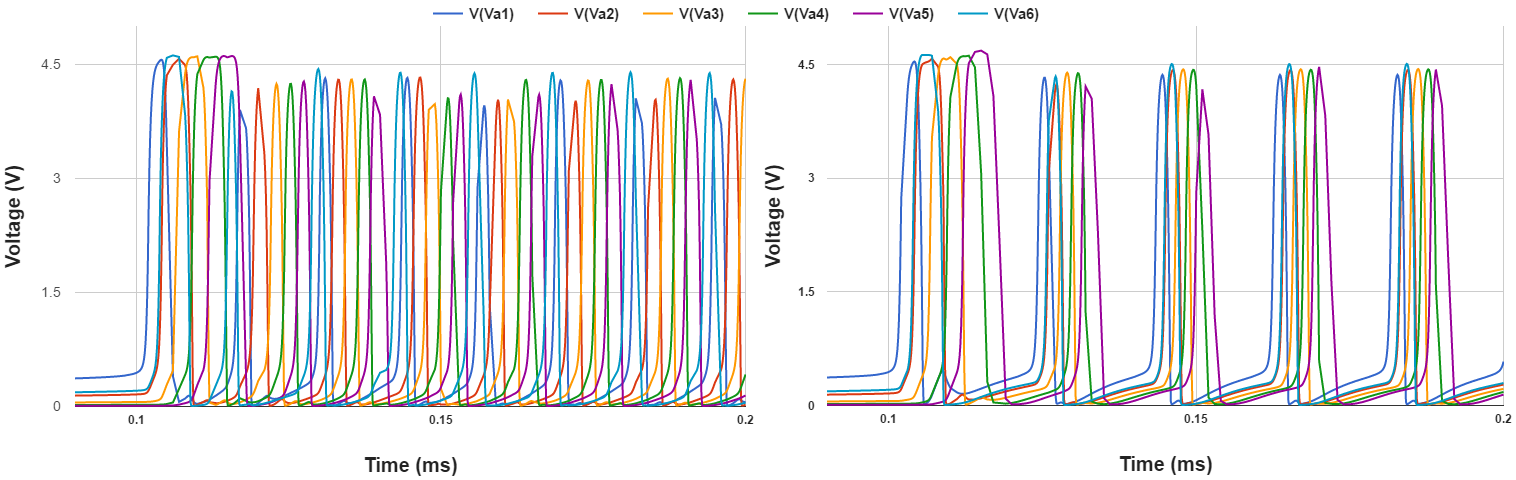
\includegraphics[width=\textwidth]{images/Electronic6cell.png}
    \caption{Left: The simulated output of voltmeters placed at positions $V_a$ (the membrane potential) in figure \ref{fig3.4} for cells 1 through 6 in figure \ref{fig3.6} in the presence of a uni-directional blocker between cells 6 and 5. Right: The same output for cells 1 through 6 in the presence of an omni-directional blocker between cells 6 and 5.}
    \label{fig3.8}
\end{figure}

One treatment for re-entrant tachycardia is ablation. This is where the uni-directional blocker is destroyed via the surgical placement of catheters and radio-frequency irradiation. The destruction of the abnormal cells transforms the uni-directional blocker into an omni-directional blocker. In the circuit model this is achieved by opening the series switch between cells 6 and 5. This stops the re-entrant current, curing the tachycardia and returning the pulse rate to normal, as shown in figure \ref{fig3.8}. 

\subsection{Further Development of the Electronic Model}
The three transistor electronic model described above is clearly limited in complexity and scale. The action potential is also not an accurate simulation of a cardiac action potential as it lacks a calcium ion controlled plateau phase. The model, in theory, could be expanded into a cubic 3D lattice or even hollow spherical structure to better simulate the heart's geometry. However, the model would start to suffer anisotropy issues as the cell circuits are designed in a linear arrangement. \par

The linear limitations of the model, as well as the action potential shape, better suit it for use in modelling nerve axon potentials. Manipulating the circuit to create an action potential more reminiscent of a cardiac action potential will require different components. Due to the limitations of using generic electrical components, this involves redesigning the circuit for every parameter change. As such we terminated development of the model here and pursued a computational path.
%---------------------------------------------------------------------------%
\newpage
\section{Computational Model}
    \label{section4}
Transitioning to a computational model provided us with the tools necessary to explore larger systems and gave us greater control over the individual cell action potentials. With the goal to create a lightweight model that effectively models the action potential of each cell; we committed to using a FN equation to model each individual cell in a homogeneous cubic lattice. This ignores the anisotropy in the biological system but dramatically reduces the computational cost. \par

The lack of anisotropy is justified as the model is designed to simulate a small section of right atrial tissue. In tissue, on this scale, the fibre structure that causes the anisotropy is heavily interconnected so can largely be ignored. When scaling up, this anisotropy could be easily included by applying a matrix to the equation which acts as a tensor. This tensor could be as simple as a scalar factor applied in each different direction of propagation or more complex to include further geometric effects. \par
The full commented code can be found in the appendix \ref{appendix2D}.

\subsection{FN Model of an Isolated Cell}
\label{sectionisocell}
Our computational model uses a FN equation based on the three transistor circuit model as described in section \ref{section3} \citep{3transistor}. Each cell's action potential ($u$) is controlled by a gating variable $v$ with the parameters $a$, $b$ and $\epsilon$ controlling the shape of the action potential curve. The initial activation potential is a function of time, $t$, as $s(t)$. The equationss take the form of
\begin{equation}
    \begin{split}
        & \frac{du}{dt}=u(u-a)(1-u)-v+s(t) \\
        & \frac{dv}{dt}=\epsilon (u-bv)
    \end{split}
    \label{eqmodel}
\end{equation}
and $u$ is plotted against $t$ to give the action potential. For the initial cell (the simulated SAN) the parameters $a, b$ and $\epsilon$ are given the values 0.15, 2.5 and 0.01 respectively. Also to simulate the external driving force that triggers the heart beat the $s(t)$ term is given a value of 0.06 for a small pulse duration (5 dimensionless time units). These parameters create an action potential as shown in figure \ref{fig5.2b}. This action potential is very similar to the action potential seen in SAN cells and as such will be used as the initial cell's action potential in our full model. \par

All values are dimensionless but an estimate of their equivalent values can be made using the multiplication factors in table \ref{tabdimensionless}. It is also important to note that dimensionless time, $t$, is sampled in steps. The sample rate set in these simulations is set at a value of 6, meaning that each dimensionless time unit is made up of 6 individual time 'steps'.

\begin{table}[H]
    \centering
    \begin{tabular}{||c c c||} 
 \hline
 Cell & membrane potential (mV) & t (s) \\ [0.5ex] 
 \hline\hline
 SAN & $(u\times94.4\pm 2)-55$ & $\times1.2\pm 0.3$\\ 
 \hline
 Atrial & $(u\times67.0\pm 2)-80$ & $\times0.5\pm 0.15$\\
 \hline
    \end{tabular}
    \caption{Multiplication factors to estimate equivalent values of the membrane potential and time from the model output.}
    \label{tabdimensionless}
\end{table}

\subsection{Propagation Mechanism}
To propagate the signal through the medium and simulate the travelling wavefront we must create a method of activating neighbouring cells. To do this we create a homogeneous cubic lattice of cells where each cell checks its nearest neighbours action potential, $u$, after a delay time, $d$, which represents the diffusion time of the extracellular ions between cells. This delayed potential of the first cell becomes the activation potential ($s(t)$) of the second. As such, the second cell's equations relative to the first can be described as
\begin{equation}
    \begin{split}
        & \frac{du_2}{dt}=u_2(u_2-a)(1-u_2)-v_2+u_1(t-d) \\
        & \frac{dv_2}{dt}=\epsilon(u_2-bv_2)
    \end{split}
\end{equation}
were $u_2$ is the action potential of the second cell and $u_1(t-d)$ is the action potential of the first cell at time $t-d$. \par

When the previous cell's action potential is passed on in this way to the next (with the same parameters as indicated in section \ref{sectionisocell}) the action potential becomes more like a square wave. This is shown in figure \ref{fig5.2b} and is very similar in shape to an atrial cells action potential. This is then propagated in a similar way across the full geometry.

\begin{figure}[H]
    \centering
    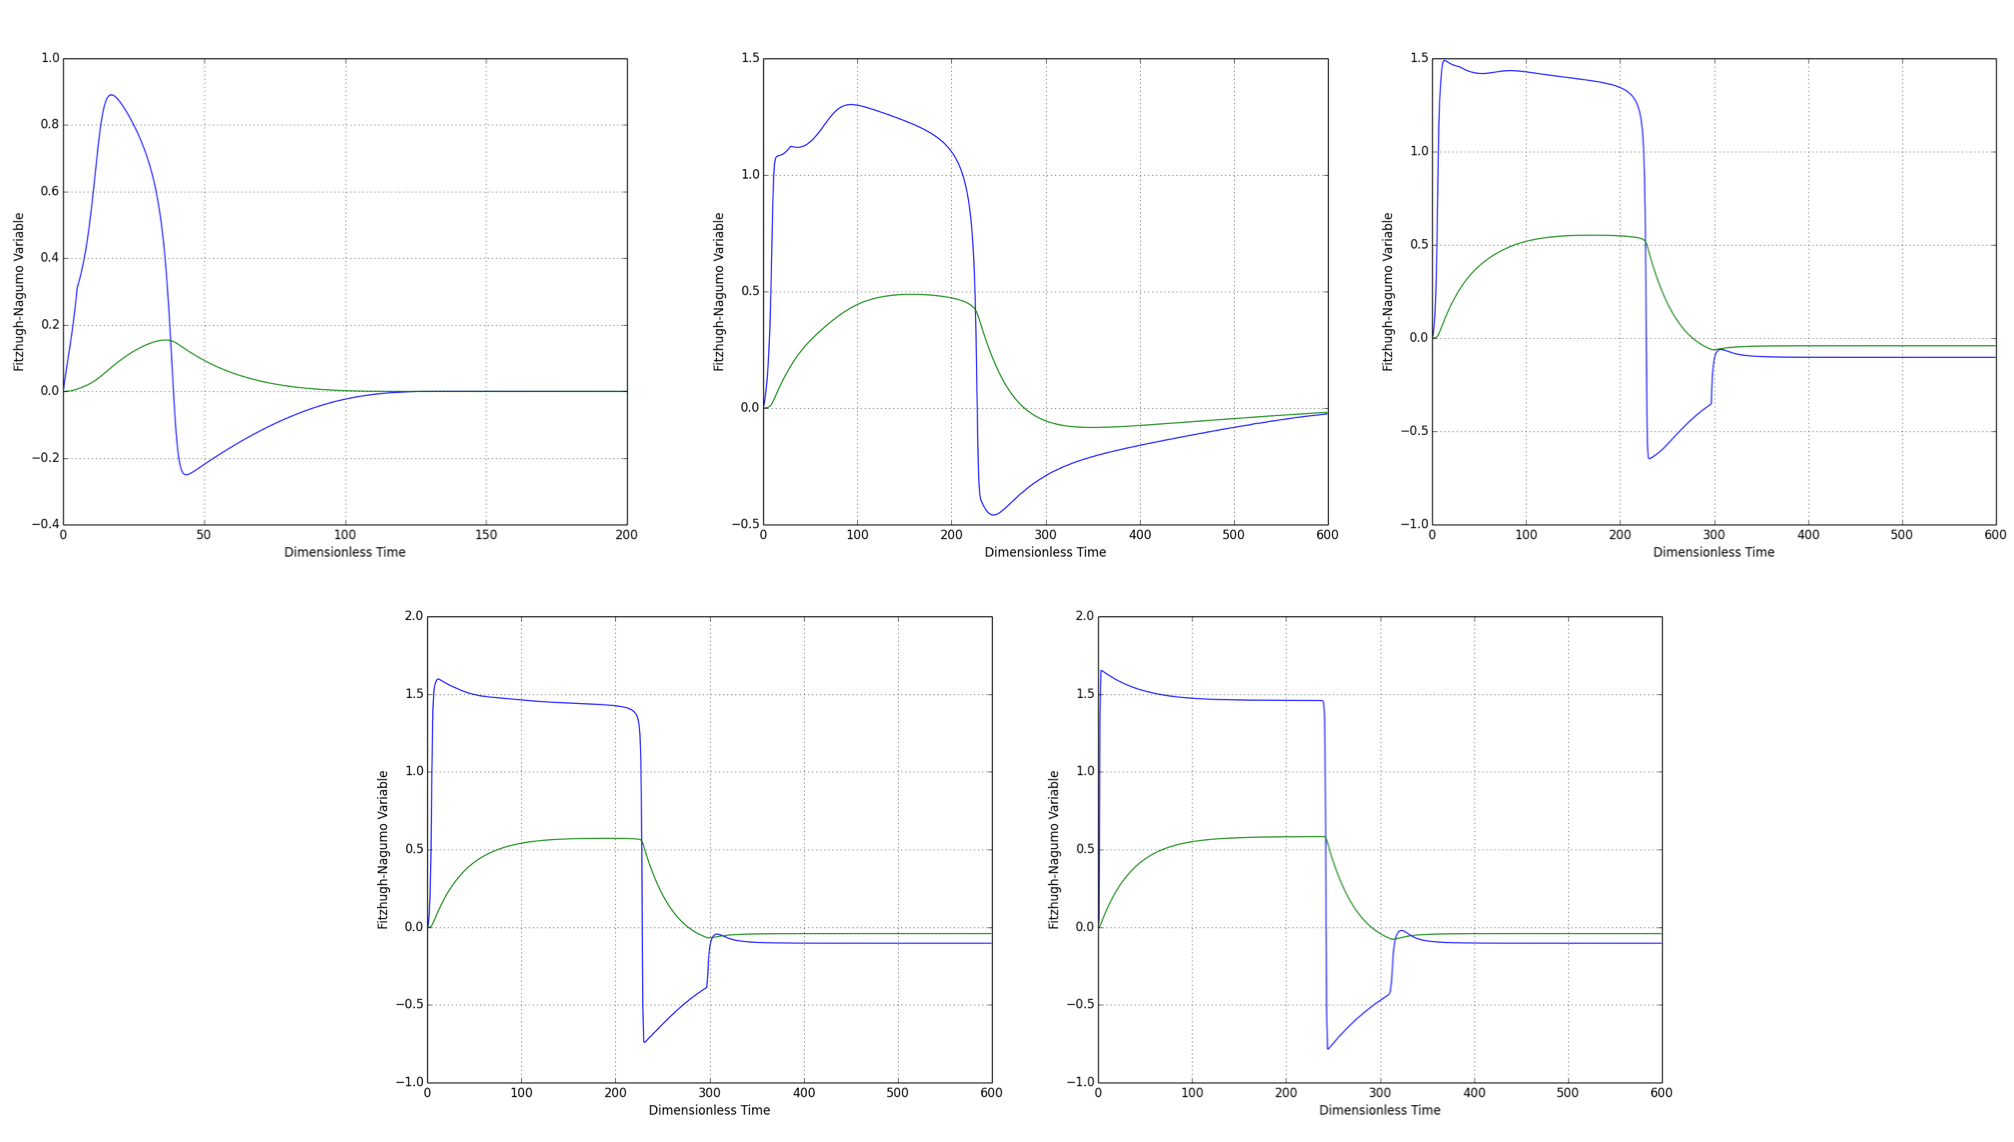
\includegraphics[width=\textwidth]{images/cellpotentials.png}
    \caption{Membrane potential outputs for a SAN cell, a $1^{st}$ column cell, a $2^{nd}$ column cell, a $3^{rd}$ column cell and a $30^{th}$ column cell (top left to bottom right). The blue and green lines show the membrane potential and gating variable respectively. The SAN output is very similar to a typical SAN cell membrane potential as shown in figure \ref{fig2.6}. The output then morphs into more of a square wave potential which can be used to model the atrial cells with the output resembling an exaggerated version of figure \ref{fig2.5}.}
    \label{fig5.2b}
\end{figure}

\subsection{2D Simulation}
In two dimensions on a 81 by 81 grid of cells, a simulation over 1800 dimensionless time units takes approximately 2 hours on a single thread of a 2.4Ghz Intel i5 processor. The code could be adapted for multi-threading and larger more complex geometries used, however, for proof of concept and functionality all following 2D simulations are carried out with these parameters. A tool for graphically displaying the output binary files can be found in appendix \ref{appendix2D}.\par

For a single beat across the geometry the first column of the matrix (x-coordinate equal to zero) is given an excitation pulse of 0.06, as described in section \ref{sectionisocell}, to simulate SAN activation. This can be expanded further to allow multiple beats as shown in figure \ref{fig5.3a}. \par
\begin{figure}[H]
    \centering
    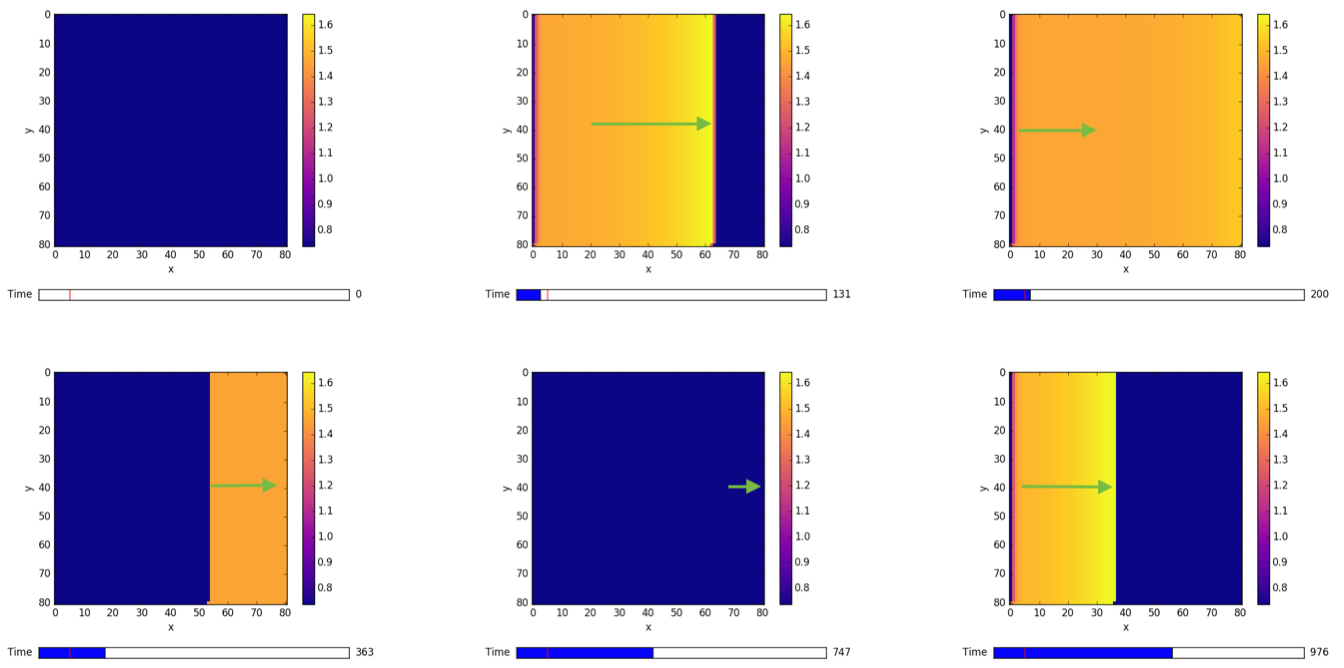
\includegraphics[width=\textwidth]{images/2beatimage.png}
    \caption{A two beat simulation with the parameters detailed in section \ref{sectionisocell}. The $x=0$ column was used as the SAN and given an initial excitation pulse of 0.06 for 5 dimensionless time units, the first at $0\leq t \geq 5$ and the second at $150 \leq t \geq 155$. The sample rate (effectively the diffusion time) is 6. The green arrows show the wavefront propagation direction. It is clear that the wavefront travels uniformly and the system relaxes as expected ready for sequential excitations.}
    \label{fig5.3a}
\end{figure}

    \subsubsection{Re-entrant Tachycardia}
    One of the causes of re-entrant tachycardia is the presence of a uni-directional blocker as described in section \ref{section2.4}. Uni-direction blockers can be simulated in our model. A uni-directional blocker blocks propagation in the positive $x$ direction but allows propagation in the negative $x$ direction. This can delay the signal for long enough to allow cells to relax and re-excite as shown in figure \ref{fig5.3.1a}. This re-entry can cause spiral waves to occur causing multiple re-excitations and thus a faster heart rate. \par
    \begin{figure}[H]
        \centering
        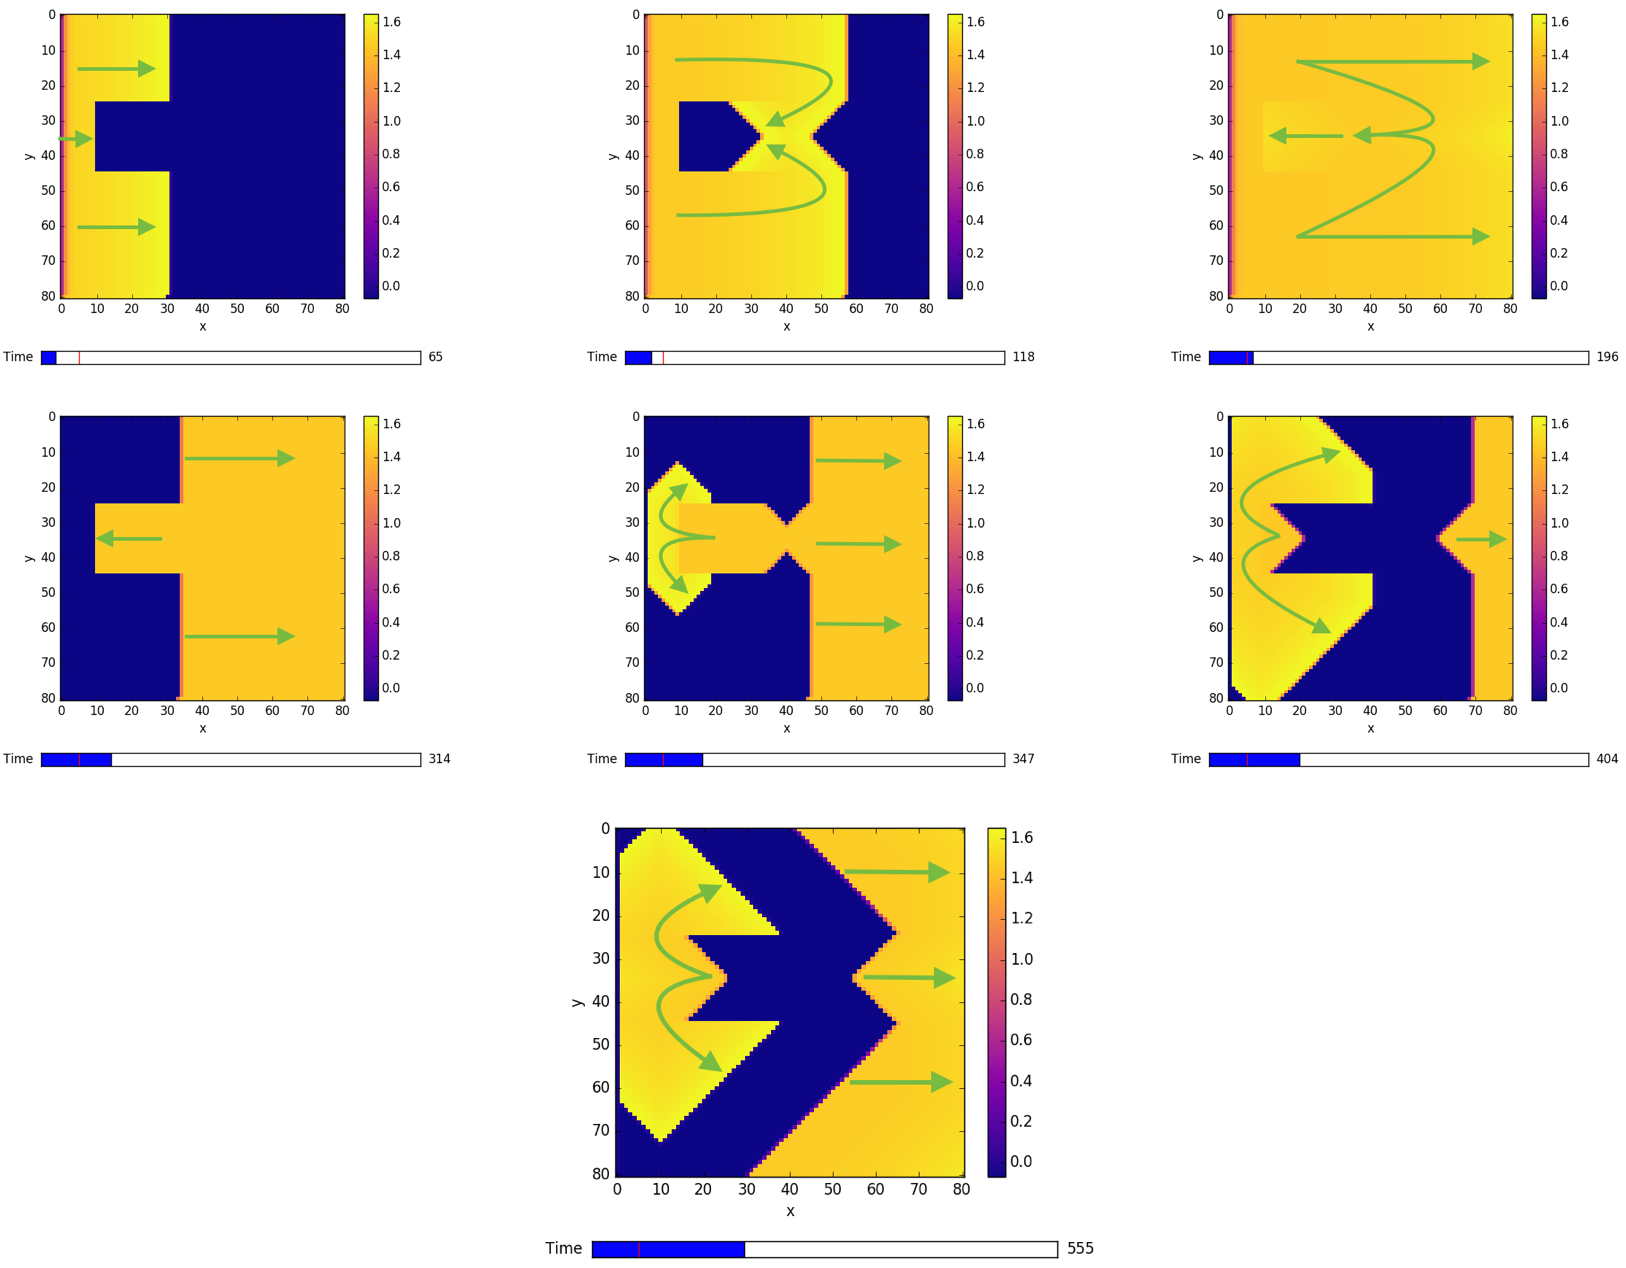
\includegraphics[width=\textwidth]{images/uniblocker.png}
        \caption{The $x=0$ column was used as the SAN and given an initial excitation pulse of 0.06 for 5 dimensionless time units at $t=0$. The sample rate (effectively the diffusion time) is 6. The green arrows show the wavefront propagation direction. The uni-directional block is a rectangle located at (10, 25) to (30, 45). Initial forward propagation is halted at the blocker, the wavefront passes the blocker and propagates back through it in the negative $x$ direction. After a period of time the cells at the forward edge of the blocker relax to a point where they can be re-excited. This allows re-entry and the wave front to re-propagate across the medium. Theses shorter echos cause the whole medium to excite simulating the effects of tachycardia.}
        \label{fig5.3.1a}
    \end{figure}
    
        \subsubsection{Ablation}
        One regularly used treatment for this kind of re-entrant tachycardia is to destroy the tissue of the blocker, effectively transforming the area from a uni-directional blocker to an omni-directional blocker. The surgical way of achieving this is via ablation, \citep{ablation2}. Ablation typically involves the use of a catheter which is used to apply radiofrequecy radiation to the effected area killing the tissue \citep{ablation}. The omni-directional blocker created does not allow backwards (negative $x$ direction) propagation so re-entry does not occur causing an end to the tachycardia.
        \begin{figure}[H]
            \centering
            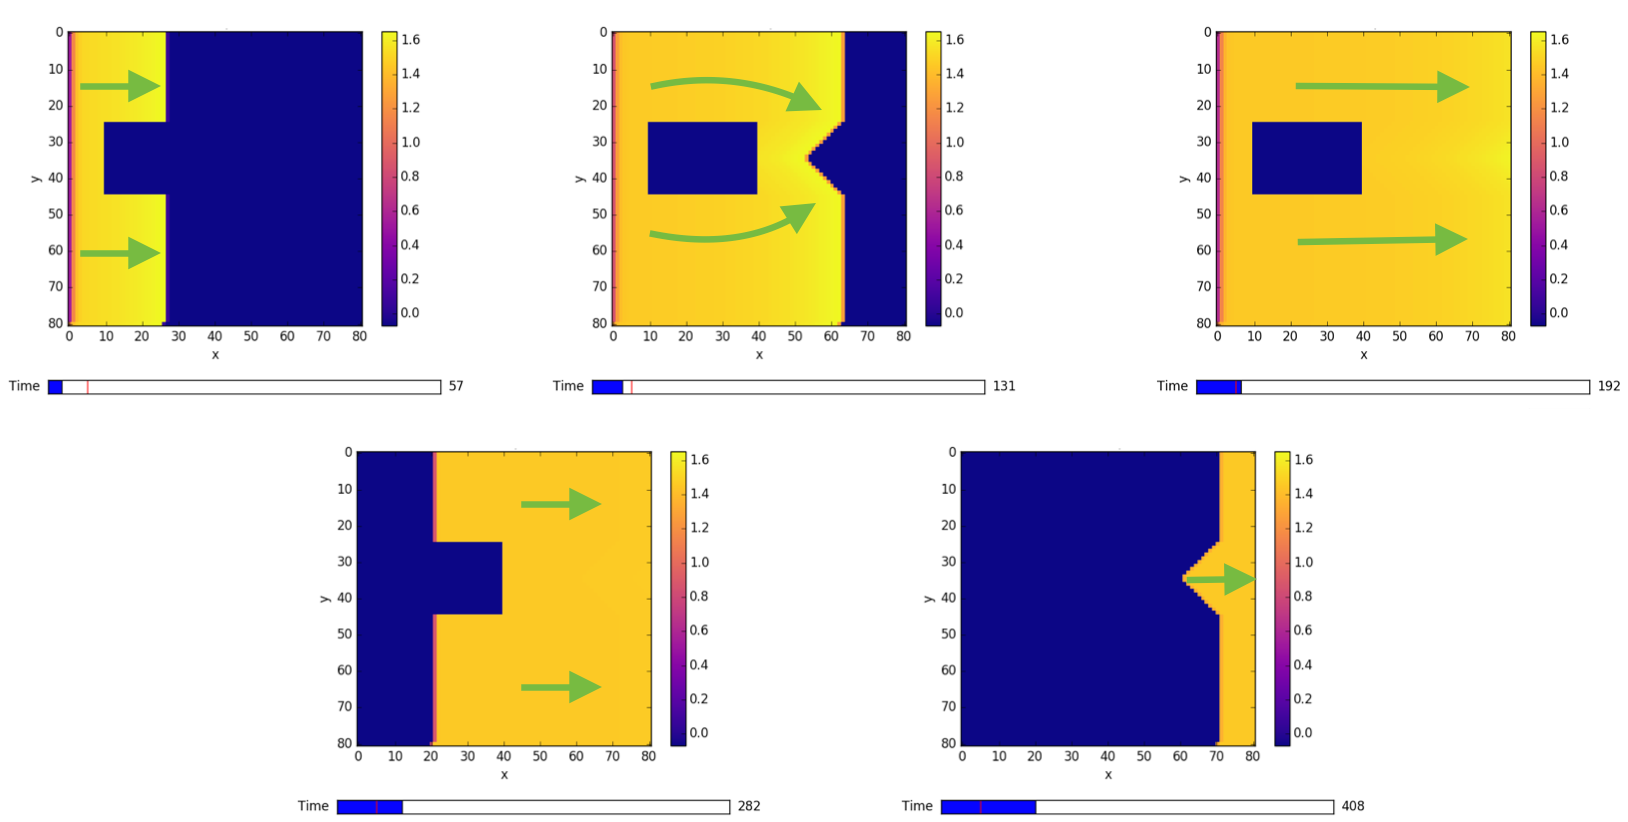
\includegraphics[width=\textwidth]{images/ablationfull.png}
            \caption{The $x=0$ column was used as the SAN and given an initial excitation pulse of 0.06 for 5 dimensionless time units at $t=0$. Sample rate is 6. Green arrows show the wavefront propagation. The omnidirectional block is a rectangle located at (10, 25) to (30, 45). Propagation is stopped in all directions by the blocker so the signal cannot propagate though the region. This does not allow any re-entry effects to occur keeping the beat rate normal.}
            \label{fig5.3.2a}
        \end{figure}

        \subsubsection{Drug Treatment}
        An alternative approach to surgical treatments is a pharmaceutical method to managing arrhythmias. Membrane ion channels and receptors are the key targets of these drugs. As previously identified; the Ca$^{2+}$, K$^+$ and Na$^+$ ion channels are vital in the generation of cardiac action potentials. \par 
        Conduction in the SA and AV nodes is dependent on Ca$^{2+}$ ion channels, therefore, Ca$^{2+}$ channel blocking drugs, such as lacidipine \citep{drugs}, are specific to arrhythmias in these regions. In other regions such as the atrium, the conduction is controlled mostly via the Na$^+$ currents and thus Na$^+$ channel blocking drugs are potentially the most effective agent. Both the Na$^+$ and Ca$^{2+}$ ions contribute to the inward current during the plateau period and as such blocking either channel would prolong the action potential duration potentially preventing re-entry.\par
        The K$^+$ ion channels contribute mainly to the repolarisation phase, as such, blocking these channels can potentially increase the action potential duration and the refractory period. The increased duration and refractory period can prevent cells from being re-excited by re-entrant effects from uni-directional blockers. This is shown in figure \ref{fig5.3.3b} where the effect of a K$^+$ channel blocking drug, such as Amidarone \citep{drugs}, was simulated by reducing the $b$ parameters in equation \ref{eqmodel} to 0.5. This reduces the gating variable's growth rate effectively reducing the repolarisation rate and thus simulating the effect of blocked K$^+$ channels.\par

        \begin{figure}[H]
            \centering
            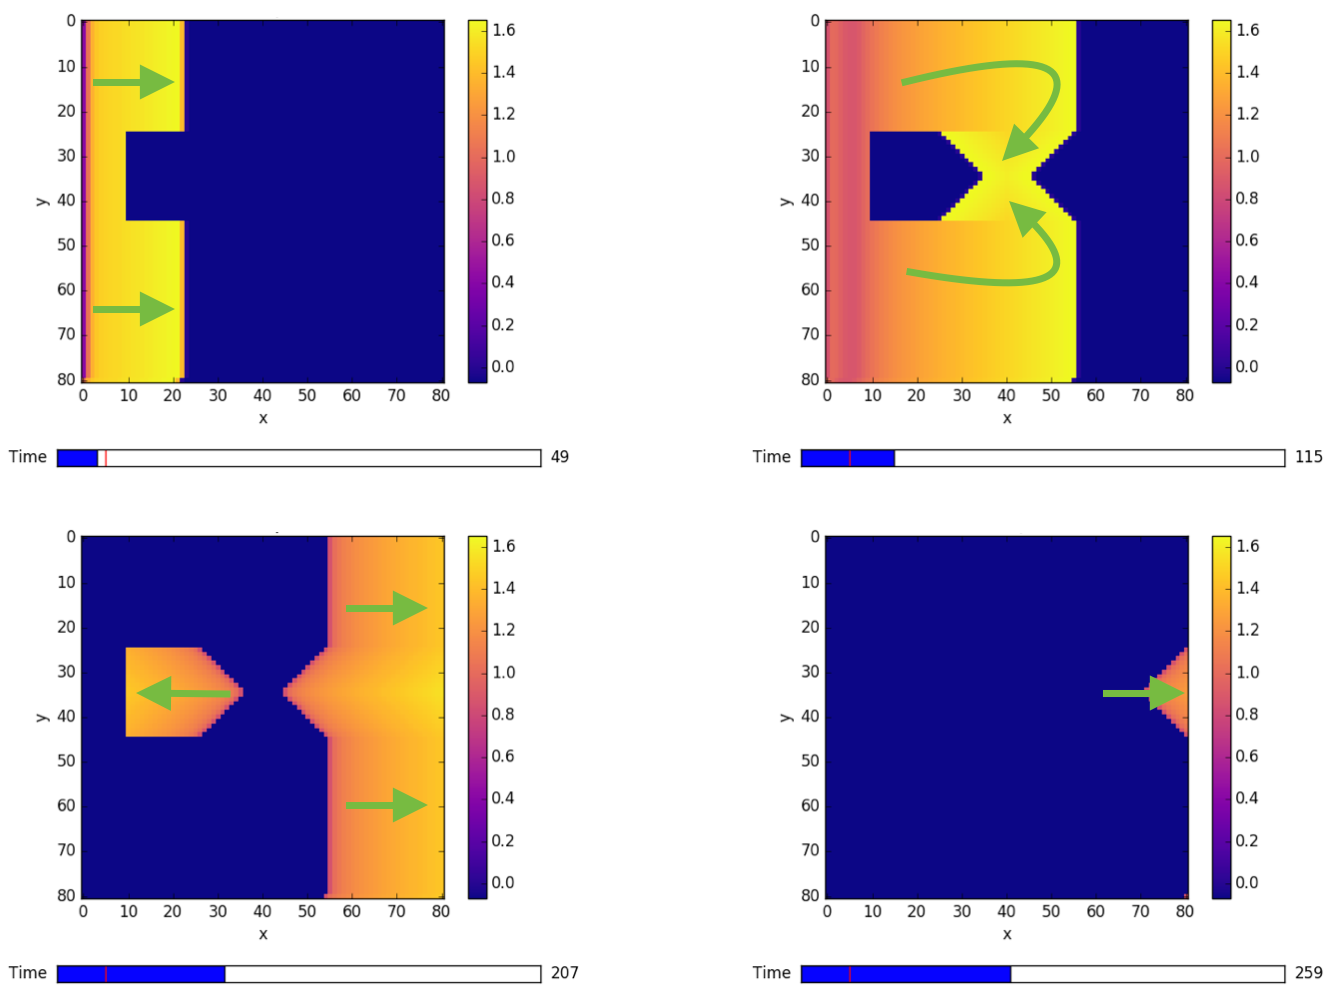
\includegraphics[width=0.8\textwidth]{images/kblock.png}
            \caption{The $x=0$ column was used as the SAN and given an initial excitation pulse of 0.06 for 5 dimensionless time units at $t=0$. Sample rate is 6. Green arrows show the wavefront propagation. Unidirectional block is a rectangle located at $(10, 25)$ to $(30, 45)$. The parameter $b$ is set to 0.5 decreasing the repolarisation phase simulating the effect of K$^+$ ion channel blocking drugs. The wavefront propagates around the unidirectional block and back propagates as before, however, due the the extended refractory period the cells do not re-excite preventing re-entry so no tachycardia is seen.}
            \label{fig5.3.3b}
        \end{figure}
        
        As the simulation is on the cellular level, there is the potential for a more advanced version of this model to be used for novel drug dosing simulation. 
        
\subsection{3D Simulation}
All simulations above have been carried out in a 2D cubic lattice geometry. Due to how the model is constructed it is trivial to add an additional dimension and expand to a 3D geometry. No simulations in 3D space have been included in this document as in a homogeneous lattice the 3$^{rd}$ dimension has very little effect on the outputted heat maps. The 3D system could be used to model more complex geometries, such as hollow ellipsoids, which more accurately represent the geometry of the atrium. A 3D model could also be modified to plot an average atrial potential against time graph, effectively modelling the P wave for comparison with diagnostic ECGs.
%---------------------------------------------------------------------------%
\newpage
\section{Discussion}
    \label{section5}
The 3 transistor electronic model exhibited in section \ref{section3} created an accurate representation of a self exciting action potential, reminiscent of a SAN cell action potential as shown in figure \ref{fig3.5}. It was also shown that these individual 3 transistor `cells' can be connected together to simulate a larger system. 6 were connected in a ring and where shown to propagate the action potential around the circuit with a diffusion time between each cell, as shown in figure \ref{fig3.7}. This method of propagation is not biologically accurate but can be used to simulate the effects of tachycardia by introducing a diode and a switch in parallel between the cells. When the switch is opened, re-entry could be simulated causing arrhythmic effects as shown in figure \ref{fig3.8}. RF ablation treatment was also simulated by transforming the unidirectional block caused by the diode into an omnidirectional block by breaking the circuit with an additional switch (figure \ref{fig3.8}). \par
The electronic model, although simple, is very restrictive. The action potential shows the relevant depolarisation and repolarisation phases with a refractory period but neglects the plateau period which is so crucial for cardiac action potentials. Being a physical circuit means that large geometries become very difficult to build and measure. Individual parameters are also very hard to control due to the limit of the components available and cost. \par
The FN type equation (equation \ref{eqmodel}) derived from the 3 transistor model showed to be effective at generating a cardiac action potential for SAN cells. The simulated SAN action potential shows all the features on a typical SAN action potential as detailed in section \ref{section2} with an accurate shape. This is significant as it does so with a very simple, lightweight method and achieves a shape that matches experimental measurements as well as other more sophisticated models. Passing the output to sequential cells causes the output to merge into more of a square wave reminiscent of atrial cell potentials. The atrial output slowly evolves over 3 cells into a stable shape, the first few cells in the sequence create an intermediary output. Although the simulated atrial potential is not as accurate a shape as the simulated SAN potential, it shows all the key features detailed in section \ref{section2} at a fraction of the computational cost of more sophisticated models. \par 
This is an important result as most advanced models create action potentials that are of similar shape and, as shown in figure \ref{fig2b.5}, vary significantly with the variable experimental measurements. These advanced models are also usually based on animals rather than humans (see table \ref{ventmodletable}). Despite these issues these advanced models are still appropriate for modelling human electrophysiology. Our model achieves a similar level of accuracy in the features of the cardiac action potential as well as overall shape for both the SAN and atrial cells but at a fraction of the computational cost, particularly in comparison to the highly detailed MCZ model \citep{phdpaper}. The model has shown to accurately simulate both individual cell electrophysiology as well as propagation mechanisms and behaviours across a variable medium. \par
The SAN and first atrial cell exhibit a gradual recovery to the resting potential which is biologically accurate, however, subsequent cells lose this gradual recovery. Instead after the restitution period they immediately recover to the resting potential. This has not caused any observable unexpected effects on the conditions simulated. This restitution period is adjustable by manipulating equation \ref{eqmodel}. \par
The model shows reliable 2D wavefront propagation which interacts as expected with uni and omnidirectional blockers, however, in its current form the code does not facilitate diagonal propagation. This addition has been made in the code but in its current state is not optimised so has been emitted from simulation. The current 2D propagation model effectively simulates re-entry of the wavefront and the establishment of spiral waves in the case of the unidirectional blocker. \par
The re-entry effect spiral waves do not interact correctly with subsequent beats from the SAN in the 81 by 81 geometry. The position of the blocker, being close to the SAN, is not allowing the cells in the first few columns time to relax and thus blocking the propagating of subsequent beats. It is believed that in larger geometries this problem can be largely negated. \par
A major advantage of this computational model in comparison to many of the models discussed in literature \citep{phdpaper} is its mathematical simplicity, and thus low computational power required. Despite being so lightweight in comparison, the model has shown accurate simulation of action potentials and wavefront propagation comparable to that of the more thorough complex models. This simplicity allows the model to simulate each individual cells action potential rather than using a finite element method. \par 
Modelling each individual cell has enabled us to be able to change the properties of the equation to simulate the effect of drugs and has shown to be effective in modelling the effect of K$^+$ ion channel blockers. This model upon further refinement could be used to simulate full scale geometries, conditions, cell types, and anisotropy. This potentially could be used for individually tailored drug dosing estimates on low powered computers, by scaling to full scale geometries and using dimensional multiplicative constants to provide estimates of the extent of treatment required to halt re-entry. The current model is not optimised for multithreading and yet simulates on the scale of hours, in comparison to a typical monodomain model which runs with an average simulation time of up to 2 days on a 32 processor computer \citep{monodomain}. \par
%---------------------------------------------------------------------------%
\section{Conclusion}
    \label{section6}
Cardiac action potentials are a complicated electrophysiological system driven by ion movements across cell membranes in the heart. They are key to understanding many cardiac conditions such as re-entrant tachycardia. It is shown that Fitzhugh-Nagumo equations can be used to model cardiac action potentials via phase-plane analysis. It is also shown that Fitzhugh-Nagumo models are mathematically lightweight in comparison to more rigorous models such as bidomain models. \par
A Fitzhugh-Nagumo system can be achieved by modelling cellular ion channels using simple electronic circuits. It is shown that a 3 transistor circuit model can be used to simulate basic action potentials and re-entrant tachycardia as well as ablation treatment. The electronic model is improved upon by taking a FN equation for the 3 transistor model and modelling a matrix of cells computationally. This system allows accurate propagation of the action potential across a geometry as well as simulation of the re-entry effect and treatment via ablation. It is also shown that the parameters of the equations can be adjusted to simulate the effects of ion channel blocking drugs. \par
In comparison to other models the FN system described is incredibly lightweight and yet could easily be adapted to include some of the more advanced simulation parameters such as anisotropy. As each cell is simulated individually the model avoids relying on finite element methods and the assumptions that are made with them. The model, with refinement, could potentially be used to accurately simulate more conditions as well as personalised drug dosing and other treatments on a cellular level while still considering the large complex geometries of the system.
%---------------------------------------------------------------------------%
\newpage
\bibliographystyle{unsrt}
\bibliography{references}
%---------------------------------------------------------------------------%
\newpage
\section{Appendix}
    \label{appendix1}
    \subsection{Nernst-Plank Equation}
\label{appendixNPE}
Ion flux across a membrane can be described by the Nernst-Plank equation. For an ion, $K$, with valance charge, $z$, the total flux can be described as the sum of the contributions of the diffusion flux $J_{diff}$ and the electric flux $J_{elec}$. $J_{diff}$ can be described by Fick's law:
\begin{equation}
    J_{diff} = -D\nabla c
\end{equation}
where $D$ is the diffusion coefficient and $c$ is the concentration of the ion. $J_{elec}$ satisfies the Plank equation:
\begin{equation}
    J_{elec} = -\frac{z}{|z|}\mu c\nabla u
\end{equation}
where $\frac{z}{|z|}$ is $+1$ for positive ions and $-1$ for negative ions, $\mu$ is the mobility of the ion and $u$ is the electric potential. \par

In both cases the ion mobility is inhibited by the presence of the solvent, as such Einstein \citep{einstien} found that $D$ and $\mu$ are related:
\begin{equation}
    D = \frac{\mu RT}{|z|F}
\end{equation}
where $R$ is the ideal gas constant, $T$ is temperature and $F$ is Faraday's constant. It follows that:
\begin{equation}
    J_{total} = J_{diff}+J_{elec} = -D\bigg(\nabla c + \frac{zF}{RT}c\nabla u\bigg)
    \label{nerstplankeq}
\end{equation}
which is known as the Nernst-Plank equation.

\subsection{Goldman-Hodgkin-Katz Current-Voltage Relation}
\label{appendixGHK}
Upon assuming $J$ and $u$ are transverse to the membrane, equation \ref{nerstplankeq} can be transformed into a linear differential equation in one dimension. 
\begin{equation}
    \frac{dc}{dx}(x)+\frac{zF}{RT}\frac{du}{dx}(x)c(x)+\frac{J}{D} = 0
\end{equation}
The solution to this can be found by multiplying by an exponential and intergrating. By then assuming the electric field is constant across the membrane of length $L$ and by using the result of the one dimensional Nernst-Plank equation the following relation can be found:
\begin{equation}
    c(x) = \frac{JRTL}{DzvF}\bigg(1-exp\bigg(\frac{zvF}{RTL}x\bigg)\bigg)+c^iexp\bigg(\frac{zvF}{RTL}x\bigg)
\end{equation}
where $v = u(0)-u(L) = u_i-u_e$. $i$ and $e$ notation is used to indicate intra and extracellular values. $c(0) = c^i$ so to satisfy $c(L) = c^e$ it follows that 
\begin{equation}
    J = \frac{DzFv}{LRT}\frac{c^i-c^eexp\big(\frac{-zvF}{RT}\big)}{1-exp\big(\frac{-zvF}{RT}\big)}
\end{equation}
By defining the electric current density $I := zFJ$ the Goldman-Hodgkin-Katz (GHK) relation is obtained.
\begin{equation}
    I=P\frac{z^2F^2}{RT}v\frac{c^i-c^eexp\big(\frac{-zvF}{RT}\big)}{1-exp\big(\frac{-zvF}{RT}\big)}
\end{equation}
where $P = \frac{D}{L}$ is the permeability of the membrane to the ion. The GHK relation is key to calculating the ion concentrations and currents discussed in section \ref{cellelectro}.

\subsection{Van Der Pol Relaxation Oscilator}
\label{appendixVDP}
First proposed in 1920 by Balthasar van der Pol, it is an oscillator with non-linear damping governed by a second order differential of the form
\begin{equation}
    \frac{dx^2}{d^2t}-\epsilon(1-x^2)\frac{dx}{dt}+x=0
\end{equation}
where $x$ is the dynamic variable (the parameter $\epsilon$ is $>0$). Using the transformation $y=x-(x^3/3)-(\frac{dx}{dt}/\epsilon)$, known as Liénard's transformation, the equation becomes
\begin{equation}
    \begin{split}
        & \frac{dx}{dt}=\epsilon(x-\frac{1}{3}x^3-y) \\
        & \frac{dy}{dt}=\frac{x}{\epsilon} \\
    \end{split}
\end{equation}
This is known as the Bonhoeffer-van der Pol model which can be electronically modelled as shown in figure \ref{fig3.2}. This circuit produces a relaxation oscillation with a period determined by the inductor and resistor. Further information can be found in the supporting literature \citep{vdp}.
\begin{SCfigure}[0.9][h!]
    \centering
    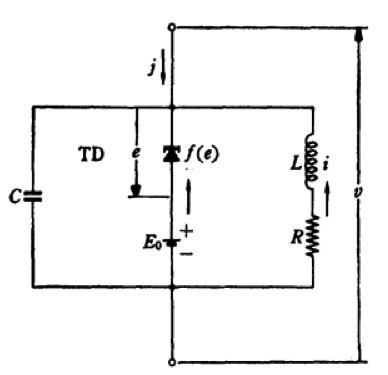
\includegraphics[width=0.4\textwidth]{images/BVP.png}
    \caption{A Bonhoeffer-Van der Pol electronic circuit, has a measured current (j) that acts as a Van der Pol relaxation oscillator. \citep{fitzhughnagumo}}
    \label{fig3.2}
\end{SCfigure}
These circuits can be coupled together to simulate a nurve axon.
\begin{SCfigure}[0.9][h!]
    \centering
    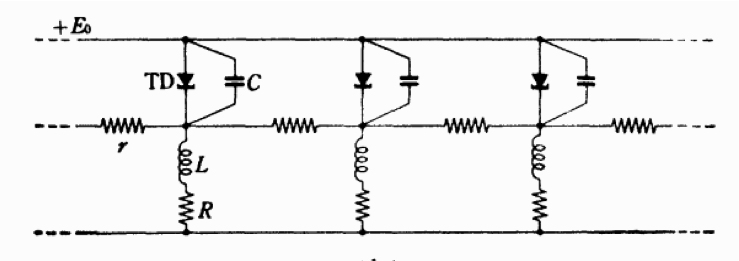
\includegraphics[width=0.7\textwidth]{images/FNaxon.png}
    \caption{A linear combination of BVP circuits (\ref{appendixVDP}) used to simulate signal propagation down a nerve axon. \citep{fitzhughnagumo}}
    \label{fig3.3}
\end{SCfigure}

\subsection{Electronic Circuit Model}
\label{appendixcircuit}
\begin{figure}[H]
    \centering
    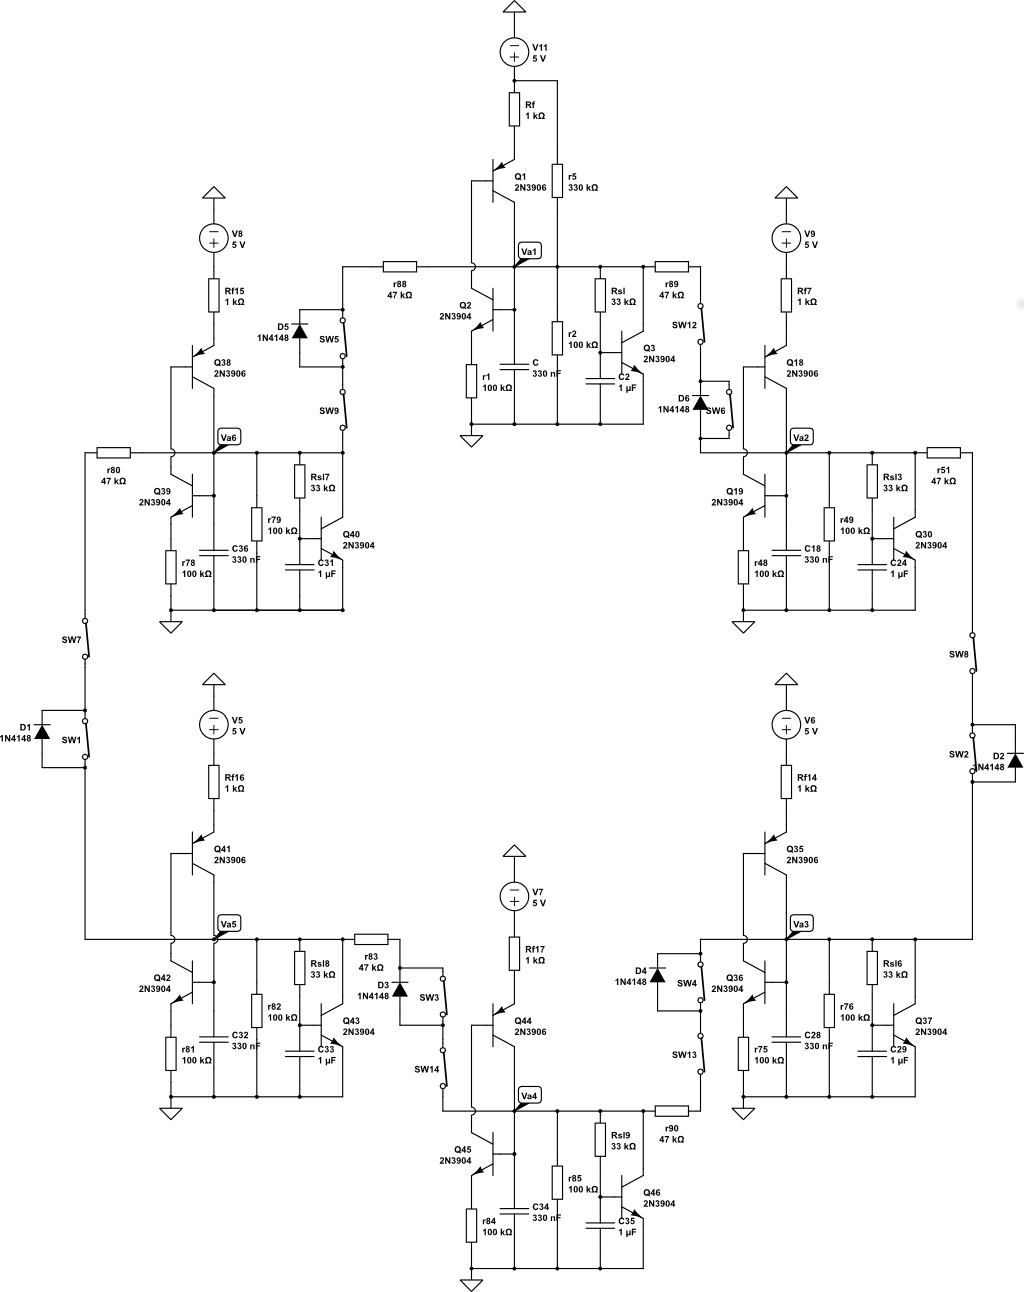
\includegraphics[width=0.9\textwidth]{images/full-circuit.png}
    \caption{A circuit diagram of 6 cells connected in a 2D ring.}
    \label{fig3.6}
\end{figure}
\begin{figure}[H]
    \centering
    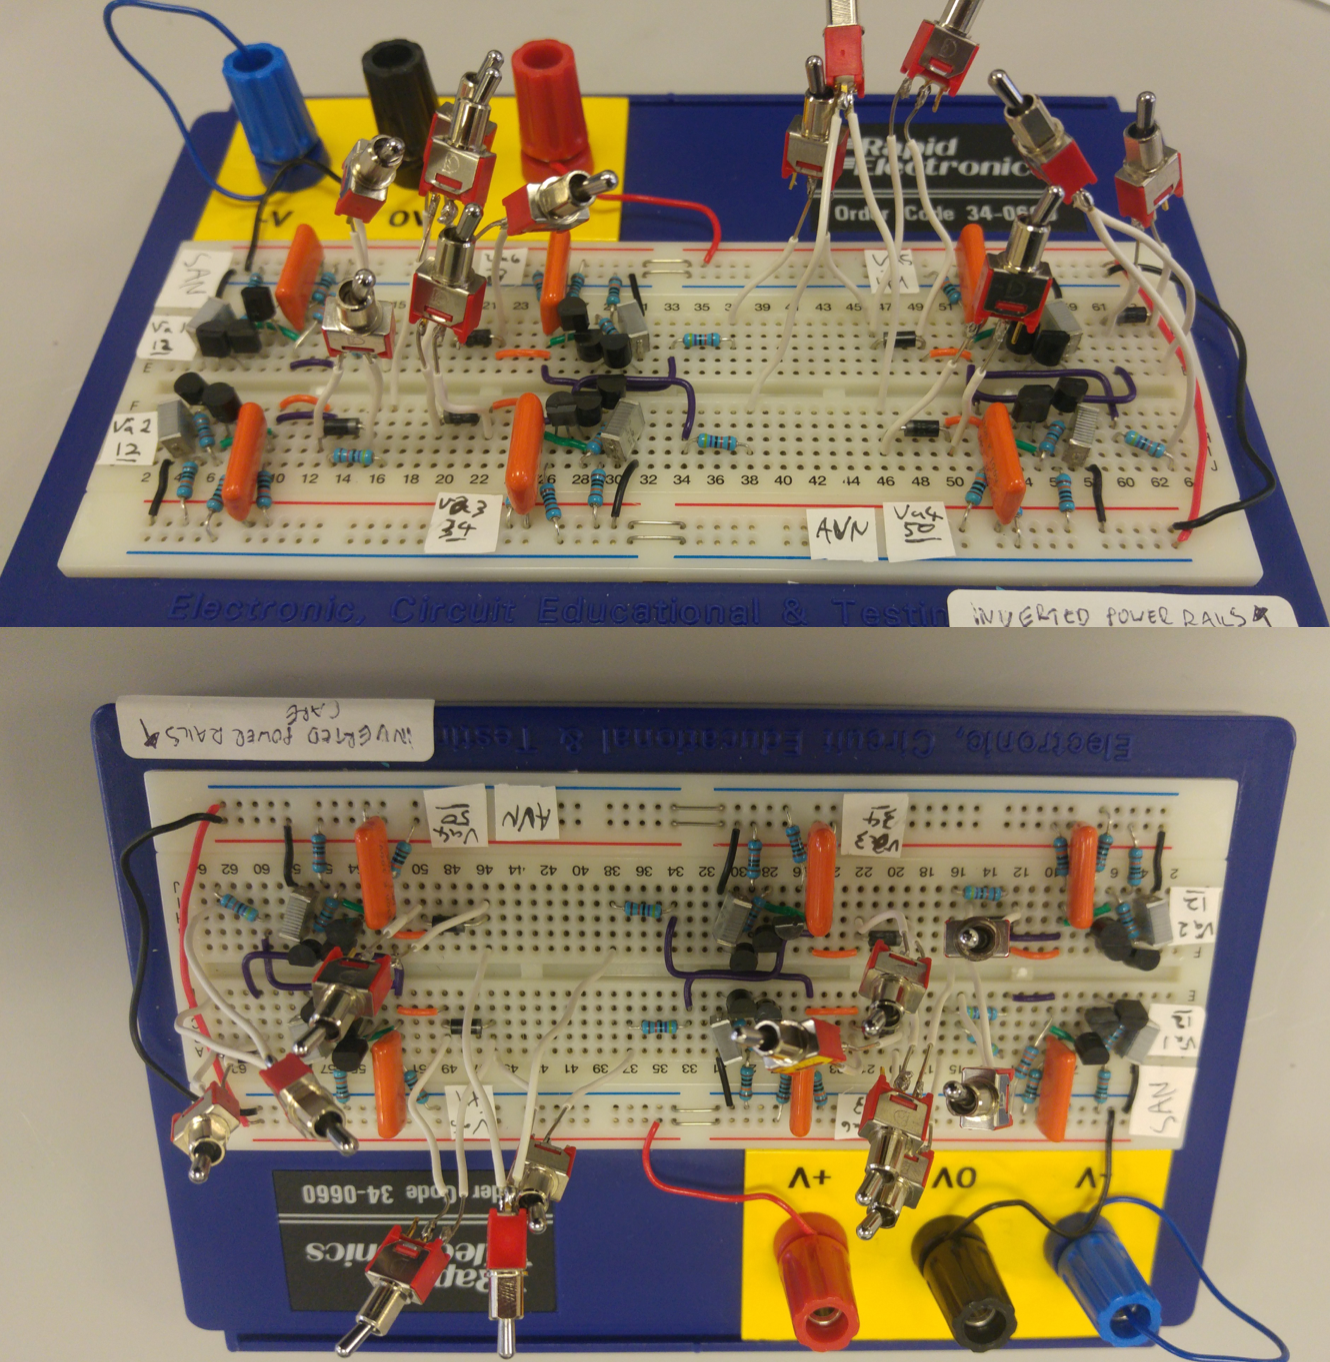
\includegraphics[width=\textwidth]{images/circuitappendix.png}
\end{figure}

\subsection{2D Code}
\label{appendix2D}
    \subsubsection{Main Code}
       \pythonexternal{main.py}
    \subsubsection{Parameters}
       \pythonexternal{param.py}
    \subsubsection{Grid Formation}
       \pythonexternal{gridCalc.py}
    \subsubsection{Solver}
       \pythonexternal{solvePlot.py}
    \subsubsection{Output Viewer}
       \pythonexternal{3dheatmap.py}

\subsection{3D Code}
\label{appendix3D}
To run the model in 3D simply add in an additional dimension to the matrix and a calculation path in the $z$ directions in the same way as $x$ and $y$ propagation are implemented.
    \subsubsection{3D Output viewer}
        \pythonexternal{4dheatmap.py}
%---------------------------------------------------------------------------%
\end{document}